% 第 9 章 向量分析与微分形式
\chapter{向量分析与微分形式}

在第 1 至第 3 节中，我们从几何的观点仔细考察向量微积分中的\newterm{divergence}{散度}{divergence}、\newterm{curl}{旋度}{curl}和\newterm{gradient}{梯度}{gradient}，引入并定义三者. 在第 4 节中，我们引入一些记号并考虑两个重要的算子——升号算子和降号算子. 理解散度、旋度、梯度与微分形式之间的关系需要这些算子，这种关系将在第 5 节中考察. 同样在第 5 节中，我们将看到线积分基本定理、散度定理和向量微积分版本的 Stokes 定理如何都能用微分形式记号写成相同的形式. 这三个定理都是所谓的广义 Stokes 定理的特殊情形. 在更高级的数学课程中，Stokes 定理总是指广义 Stokes 定理，而不是你在向量微积分中学到的那个版本的 Stokes 定理，而在物理学中，Stokes 定理可能指两者中的任何一个，取决于上下文. 但请记住，从更抽象的观点来看，它们实际上是同一个定理.

\section{散度}

在向量微积分中，$\mathbb{R}^3$ 上的向量场 $F$ 通常写成 $F=P(x,y,z)\hat{\imath}+Q(x,y,z)\hat{\jmath}+R(x,y,z)\hat{k}$，其中 $P,Q,R:\mathbb{R}^3\to\mathbb{R}$. 这里 $\hat{\imath}$、$\hat{\jmath}$ 和 $\hat{k}$ 分别是 $x$、$y$、$z$ 方向的单位向量. 如果我们把变量记为 $x_1,x_2,x_3$，那么单位向量通常写成 $e_1,e_2,e_3$. 回忆我们总是把向量写成列向量，
\[
F=\begin{bmatrix}P\\Q\\R\end{bmatrix}.
\]

在向量微积分课程中，向量场 $F$ 的散度通常定义为
\[
\operatorname{div}F=\frac{\partial P}{\partial x}+\frac{\partial Q}{\partial y}+\frac{\partial R}{\partial z}.
\]
常常定义一个算子 $\nabla$ 为
\[
\nabla=\frac{\partial}{\partial x}e_1+\frac{\partial}{\partial y}e_2+\frac{\partial}{\partial z}e_3.
\]
如果这样做，那么我们可以考虑算子 $\nabla$ 与向量 $F$ 的``点积''为
\[
\operatorname{div}F=\nabla\cdot F=\Bigl(\frac{\partial}{\partial x}e_1+\frac{\partial}{\partial y}e_2+\frac{\partial}{\partial z}e_3\Bigr)\cdot(Pe_1+Qe_2+Re_3)=\frac{\partial P}{\partial x}+\frac{\partial Q}{\partial y}+\frac{\partial R}{\partial z}.
\]
这看起来确实有点傻，因为点积需要两个向量，而显然 $\nabla$ 并不是真正的向量，它是别的东西. 它通常被称为算子，并且说它``作用于''向量 $F$. 类似地，可以把 $\nabla$ 算子想成与列向量 $F$ 做矩阵乘法的行向量，
\[
\nabla\cdot F=\Bigl(\frac{\partial}{\partial x},\frac{\partial}{\partial y},\frac{\partial}{\partial z}\Bigr)\begin{bmatrix}P\\Q\\R\end{bmatrix}.
\]
这个所谓的把 $\operatorname{div}F$ 定义为 $\nabla\cdot F$ 的定义，实际上更像是一种记忆辅助手段，帮助我们记住在使用笛卡尔坐标时 $\operatorname{div}F$ 的形式.

关于术语的一个简短说明. 符号 $\nabla$ 实际上称为 nabla，源自希伯来语中``竖琴''一词，竖琴是一种大致呈 $\nabla$ 形状的弦乐器. 当 $\nabla$ 被用来表示散度算子时，它通常被称为 del. 人们会把 $\nabla\cdot F$ 读作``del dot F''，或读作``div F''，或读作``$F$ 的散度''.

我们将在这里采取不同的方法，以一种使散度定理可以从定义中直接落出来的方式来定义 $\operatorname{div}F$. 利用这一点，我们将推导出笛卡尔坐标下 $\operatorname{div}F$ 的标准公式. 我们采取这种方法，是因为我们相信它能为散度背后的意义提供某种更几何的解释. 但在我们这样做之前，首先需要理解向量场法向分量的曲面积分是什么. 由于我们实际上假设你已经上过向量微积分课程，我们将快速且不做太多细节地介绍这些材料；我们更关心概念上的理解而不是数学上的严格性.

假设我们在 $\mathbb{R}^3$ 上有一个向量场 $F=P\hat{\imath}+Q\hat{\jmath}+R\hat{k}$，以及 $\mathbb{R}^3$ 中的一个二维曲面 $S$，如图~\ref{fig:9-1} 所示. 我们想把 $F$ 在曲面 $S$ 上的积分定义为某种东西. 从某种意义上说，我们在问有多少向量场 $F$ 穿过曲面 $S$. 如果 $F$ 表示流体粒子的速度，这就更有直观意义了. 那么我们基本上是在问流体通过曲面 $S$ 的流率. 见图~\ref{fig:9-2}.

\begin{figure}[htbp]
  \centering
  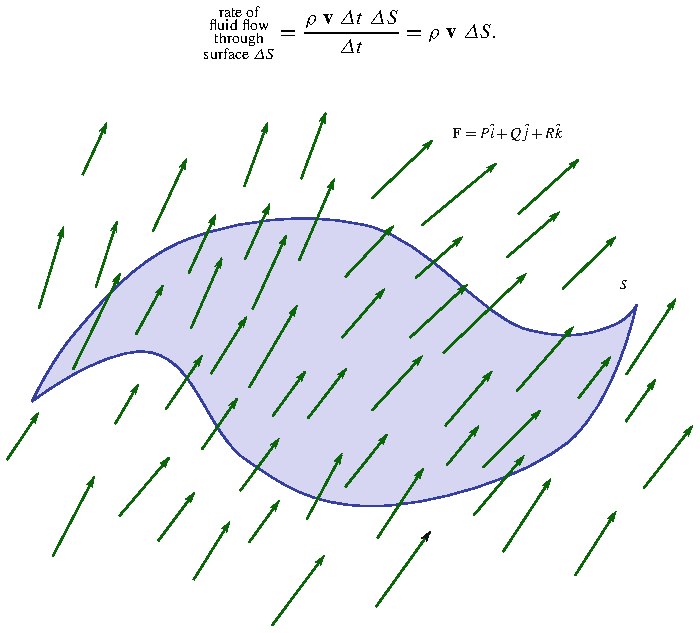
\includegraphics[width=0.832\linewidth]{images/vector/fig-9-1.pdf}
  \caption{$\mathbb{R}^3$ 中的向量场 $F=P\hat{\imath}+Q\hat{\jmath}+R\hat{k}$ 以及二维曲面 $S$}
  \label{fig:9-1}
\end{figure}

\begin{figure}[htbp]
  \centering
  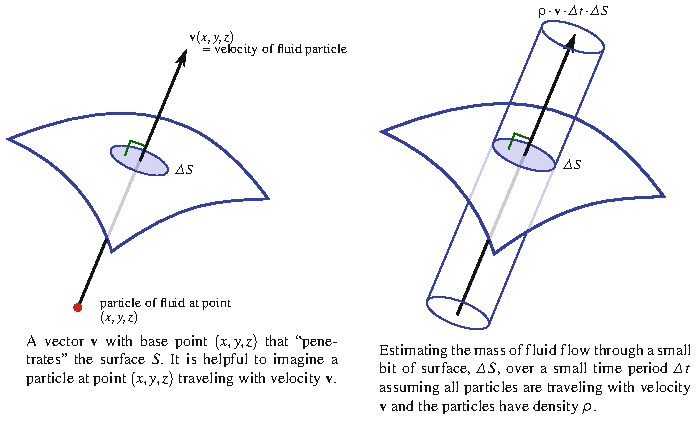
\includegraphics[width=0.827\linewidth]{images/vector/fig-9-2.pdf}
  \caption{把向量场 $v$ 在曲面 $S$ 上的积分想成求以速度 $v$ 运动并通过该曲面的流体的流率，是一种自然的思考方式}
  \label{fig:9-2}
\end{figure}

假设对于密度为 $\rho(x,y,z)$ 的某种流体，$v(x,y,z)$ 是点 $(x,y,z)$ 处的流体粒子的流动速度. 我们想求有多少流体流过某个小曲面 $\Delta S$. 如果我们假设 $v$ 垂直于 $\Delta S$，那么在一个小时间段 $\Delta t$ 内，流过 $\Delta S$ 的流体的质量由 $\rho(x,y,z)v(x,y,z)\Delta t\Delta S$ 给出，如图~\ref{fig:9-2} 所示. 流率由穿过曲面的流体质量除以这些质量穿过曲面的时间给出：
\[
\text{通过曲面 }\Delta S\text{ 的流体流率}=\frac{\rho v\Delta t\Delta S}{\Delta t}=\rho v\Delta S.
\]

如果 $v$ 不垂直于曲面 $\Delta S$，那么通过 $\Delta S$ 的流动由 $\rho(x,y,z)\,v(x,y,z)\cdot\hat{n}\,\Delta t\Delta S$ 给出. 也就是说，我们把乘积中的 $v$ 替换为 $v\cdot\hat{n}$，即与曲面元素 $\Delta S$ 的单位法向量的点积. 这个点积给出 $v$ 在 $\hat{n}$ 方向的分量. 见图~\ref{fig:9-3}. 换句话说，它给出流体在 $\hat{n}$ 方向的流动速度，
\[
\text{通过曲面 }\Delta S\text{ 的流体流率}=\frac{\rho(v\cdot\hat{n})\Delta t\Delta S}{\Delta t}=\rho(v\cdot\hat{n})\Delta S.
\]

\begin{figure}[htbp]
  \centering
  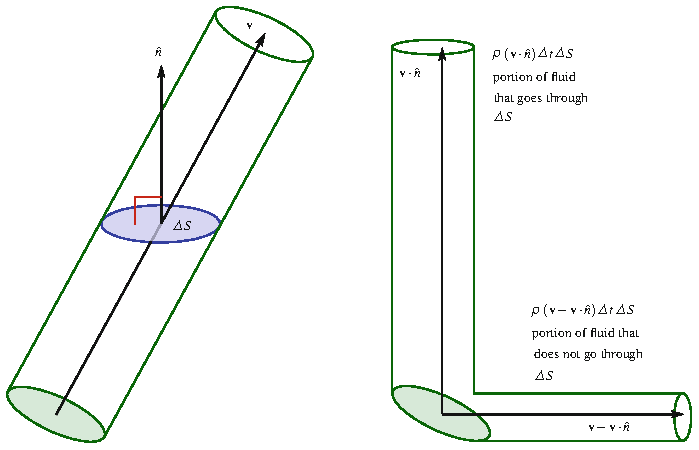
\includegraphics[width=0.960\linewidth]{images/vector/fig-9-3.pdf}
  \caption{假设 $v$ 不垂直于曲面 $S$（左）. 那么我们把流体流动``分解''成两部分：穿过曲面 $S$ 的那部分和不穿过 $S$ 的那部分（右）. 这需要取 $v$ 与 $S$ 的单位法向量（记为 $\hat{n}$）的点积}
  \label{fig:9-3}
\end{figure}

我们可以通过把 $S$ 分成小块 $\Delta S$、求每一块的流动然后求和，来近似整个曲面 $S$ 的流体流动. 然后为了求精确的流动，我们可以取 $\Delta S$ 的大小收缩到零的极限，即 $|\Delta S|\to0$：
\[
\text{流率}=\lim_{|\Delta S_i|\to0}\sum_i\rho(v\cdot\hat{n})\Delta S_i=\iint_S\rho(v\cdot\hat{n})\,dS.
\]

我们一直在处理一个具体的情形——流体流动——来帮助我们更好地理解正在发生的事情. 但同样的推理适用于任何向量场 $F$；我们可以求向量场 $F$ 穿过曲面 $S$ 的``流动''. 但是当我们拿掉流体这个心理拐杖、只处理向量场时，实际上没有流体密度 $\rho$，所以我们必须从上面的等式中去掉 $\rho$. 但在这种更纯粹的情形下，我们只有向量场而没有流体，我们实际上并不是在求流体流过 $S$ 的流率. 我们求的这个公认抽象的东西被称为向量场 $F$ 穿过曲面 $S$ 的\newterm{flux}{通量}{flux}. 通量（flux）是拉丁语中``流动''的意思. 通量在物理情形中实际代表什么取决于具体问题以及向量场被如何解释. 这个向量是流体流动？是电场？是磁场？是力？在每种情况下，穿过曲面的通量都会被不同地解释. 所以通量实际上是一个抽象数学概念，在不同的物理情形下可以被不同地解释. 稍后我们将看到场 $F$ 表示电场或磁场的例子，我们将求出穿过曲面的电通量和磁通量. 然而，一般来说，思考通量到底是什么的最好方法大概是想象一种没有密度的流体. 这样我们就有
\[
\operatorname{Flux}(F)=\lim_{|\Delta S_i|\to0}\sum_i F\cdot\hat{n}\,\Delta S_i=\iint_S F\cdot\hat{n}\,dS.
\]
注意这个积分有意义：在曲面 $S$ 上的每个点 $p$，$F_p\cdot\hat{n}_p$ 是一个实数. 也就是说，我们可以把 $F\cdot\hat{n}$ 想成 $S$ 上的实值函数，$F\cdot\hat{n}:S\to\mathbb{R}$，这意味着我们可以容易地把它在曲面 $S$ 上积分. 在向量微积分中你学过各种做这件事的技巧. 总之，向量场 $F$ 穿过曲面 $S$ 的通量由积分
\[
\operatorname{Flux}(F)=\iint_S F\cdot\hat{n}\,dS
\]
给出.

关于记号的两点说明：有时这个积分写成 $\oint_S F\cdot dS$ 或 $\iint_S F\cdot dS$. 所以当你看到 $\oint_S F\cdot dS$ 或 $\iint_S F\cdot dS$ 时，它的意思正是 $\iint_S F\cdot\hat{n}\,dS$. 这种记号将在第~\ref{sec:9-5-3}~小节中更深入地解释. 另外，由于 $S$ 是曲面而不是函数，显然 $dS$ 不代表一个 0-形式的外微分. 但 $dS$ 来自 $\Delta S$，它表示曲面 $S$ 的一小块的面积，所以粗略地你可以把 $dS$ 想成曲面 $S$ 上的一个``面积形式''，它允许你求出曲面 $S$ 的面积. 我们在这里不深入细节.

现在我们将定义 $F$ 在点 $(x_0,y_0,z_0)$ 处的散度. 假设我们有一个围绕点 $(x_0,y_0,z_0)$ 的小三维区域 $V$. 这个区域 $V$ 的边界记为 $\partial V$. 所谓闭的，我们的意思是曲面 $S$ 像一个没有边的球面. 我们还将区域 $V$ 的体积记为 $\Delta V$. 那么我们把 $F$ 的散度定义为
\begin{definition}[散度的定义]\label{def:9-1-1}
\[
\operatorname{div}F=\lim_{\Delta V\to0}\frac{1}{\Delta V}\oint_{\partial V}F\cdot\hat{n}\,dS.
\]
\end{definition}

理解这实际上代表什么可能会更容易一些，如果我们把右边写成
\[
\lim_{\Delta V\to0}\frac{\oint_{\partial V}F\cdot\hat{n}\,dS}{\Delta V}
\]
并考虑这意味着什么. 在分子中是穿过 $\partial V$ 的通量，即向量场穿过曲面 $\partial V$ 的流动. 由于 $\partial V$ 是闭曲面，如果我们选择法向量 $\hat{n}$ 指向外部，那么 $F$ 穿过 $\partial V$ 的通量就是 $F$ 流出 $V$ 的净通量减去流入 $V$ 的净通量. 换句话说，$F$ 通过 $\partial V$ 流出 $V$ 的净通量，即 $\oint_{\partial V}F\cdot\hat{n}\,dS$，可以是正的、零或负的. 把 $F$ 流出 $V$ 的净通量除以 $\Delta V$，我们求的是 $F$ 流出 $V$ 的每单位体积的净通量. 当我们让围绕点 $(x_0,y_0,z_0)$ 的体积 $\Delta V$ 的极限趋于零时，我们求出的就是在点 $(x_0,y_0,z_0)$ 处每单位体积的净流出通量. 换句话说，这就是向量场 $F$ 在点 $(x_0,y_0,z_0)$ 处``发散''的程度.

如果 $\operatorname{div}F$ 在点 $(x_0,y_0,z_0)$ 处为正，那么这意味着向量场 $F$ 正在从点 $(x_0,y_0,z_0)$ 向外发散. 如果 $\operatorname{div}F$ 在点 $(x_0,y_0,z_0)$ 处为负，那么这意味着向量场 $F$ 正在点 $(x_0,y_0,z_0)$ 处积聚. 如果 $\operatorname{div}F$ 在点 $(x_0,y_0,z_0)$ 处为零，那么 $F$ 在该点既不积聚也不发散. 见图~\ref{fig:9-4}.

\begin{figure}[htbp]
  \centering
  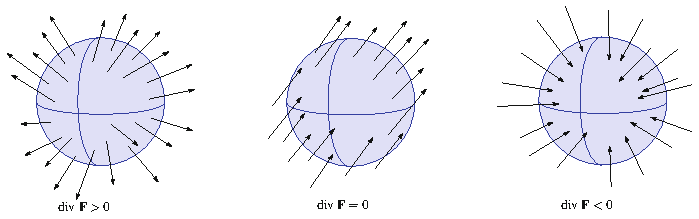
\includegraphics[width=0.960\linewidth]{images/vector/fig-9-4.pdf}
  \caption{向量场关于点 $(x_0,y_0,z_0)$ 周围小体积 $\Delta V$ 的通量的三个例子. 图中显示了通量为正（左）、为零（中）和为负（右）的情形}
  \label{fig:9-4}
\end{figure}

现在我们想用 $F$ 的散度的定义 $\operatorname{div}F=\lim_{\Delta V\to0}\frac{1}{\Delta V}\oint_{\partial V}F\cdot\hat{n}\,dS$ 来得到你在向量微积分中学过的散度标准公式 $\frac{\partial P}{\partial x}+\frac{\partial Q}{\partial y}+\frac{\partial R}{\partial z}$. 利用图~\ref{fig:9-5} 中所示的立方体区域 $V$，我们有曲面 $S_1$ 和 $S_2$，它们平行于 $y$ 轴和 $z$ 轴、垂直于 $x$ 轴. 我们把 $S_1$ 想成立方体的前面，把 $S_2$ 想成立方体的后面. $S_1$ 的朝外法向量是 $\hat{n}_{S_1}=\hat{\imath}$，$S_2$ 的朝外法向量是 $\hat{n}_{S_2}=-\hat{\imath}$. 我们有
\[
\oint_{S_1}F\cdot\hat{n}_{S_1}\,dS\approx F\Bigl(x_0+\frac{\Delta x}{2},y_0,z_0\Bigr)\cdot\hat{\imath}\,\Delta y\Delta z=P\Bigl(x_0+\frac{\Delta x}{2},y_0,z_0\Bigr)\Delta y\Delta z
\]
和
\[
\oint_{S_2}F\cdot\hat{n}_{S_2}\,dS\approx F\Bigl(x_0-\frac{\Delta x}{2},y_0,z_0\Bigr)\cdot(-\hat{\imath})\,\Delta y\Delta z=-P\Bigl(x_0-\frac{\Delta x}{2},y_0,z_0\Bigr)\Delta y\Delta z.
\]

\begin{figure}[htbp]
  \centering
  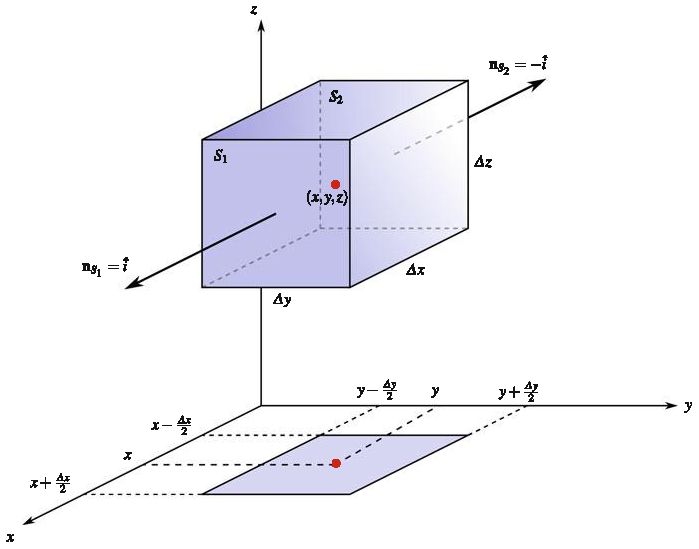
\includegraphics[width=0.960\linewidth]{images/vector/fig-9-5.pdf}
  \caption{区域 $V$ 是边长分别为 $\Delta x$、$\Delta y$ 和 $\Delta z$ 的立方体，因此 $\Delta V=\Delta x\Delta y\Delta z$. 侧面 $S_1$ 和 $S_2$（立方体的前面和后面）垂直于 $x$ 轴. $S_1$ 的朝外单位法向量是 $\hat{\imath}$，$S_2$ 的朝外单位法向量是 $-\hat{\imath}$}
  \label{fig:9-5}
\end{figure}

求和得到
\begin{align*}
\oint_{S_1+S_2}F\cdot\hat{n}\,dS\approx\Bigl[P\Bigl(x_0+\frac{\Delta x}{2},y_0,z_0\Bigr)-P\Bigl(x_0-\frac{\Delta x}{2},y_0,z_0\Bigr)\Bigr]\Delta y\Delta z \\
=\frac{P\bigl(x_0+\frac{\Delta x}{2},y_0,z_0\bigr)-P\bigl(x_0-\frac{\Delta x}{2},y_0,z_0\bigr)}{\Delta x}\Delta x\Delta y\Delta z, \\
\Rightarrow\quad\frac{1}{\Delta x\Delta y\Delta z}\oint_{S_1+S_2}F\cdot\hat{n}\,dS\approx\frac{P\bigl(x_0+\frac{\Delta x}{2},y_0,z_0\bigr)-P\bigl(x_0-\frac{\Delta x}{2},y_0,z_0\bigr)}{\Delta x}.
\end{align*}
回想 $\Delta V=\Delta x\Delta y\Delta z$，然后取 $\Delta V\to0$（即 $\Delta x\to0$、$\Delta y\to0$ 和 $\Delta z\to0$）的极限，我们得到
\begin{align*}
\lim_{\Delta V\to0}\frac{1}{\Delta V}\oint_{S_1+S_2}F\cdot\hat{n}\,dS
=\lim_{\Delta V\to0}\frac{P\bigl(x_0+\frac{\Delta x}{2},y_0,z_0\bigr)-P\bigl(x_0-\frac{\Delta x}{2},y_0,z_0\bigr)}{\Delta x} \\
=\lim_{\Delta x\to0}\frac{P\bigl(x_0+\frac{\Delta x}{2},y_0,z_0\bigr)-P\bigl(x_0-\frac{\Delta x}{2},y_0,z_0\bigr)}{\Delta x}
=\left.\frac{\partial P}{\partial x}\right|_{(x_0,y_0,z_0)}.
\end{align*}
在极限中近似变成等式. 另外，由于右边没有 $\Delta y$ 或 $\Delta z$，$\Delta V\to0$ 就简化为 $\Delta x\to0$.

\begin{question}\label{q:9-1}
令 $S_3$ 和 $S_4$ 是区域 $V$ 中垂直于 $y$ 轴的侧面，即立方体的右侧面和左侧面. 令 $S_5$ 和 $S_6$ 是垂直于 $z$ 轴的侧面，即立方体的顶面和底面. 对曲面 $S_3+S_4$ 和 $S_5+S_6$ 重复这些计算，得到
\[
\lim_{\Delta V\to0}\frac{1}{\Delta V}\oint_{S_3+S_4}F\cdot\hat{n}\,dS=\left.\frac{\partial Q}{\partial y}\right|_{(x_0,y_0,z_0)},\qquad
\lim_{\Delta V\to0}\frac{1}{\Delta V}\oint_{S_5+S_6}F\cdot\hat{n}\,dS=\left.\frac{\partial R}{\partial z}\right|_{(x_0,y_0,z_0)}.
\]
\end{question}

把所有项加在一起，我们有
\begin{align*}
\operatorname{div}F=\lim_{\Delta V\to0}\frac{1}{\Delta V}\oint_{\partial V}F\cdot\hat{n}\,dS
=\lim_{\Delta V\to0}\frac{1}{\Delta V}\oint_{S_1+S_2+S_3+S_4+S_5+S_6}F\cdot\hat{n}\,dS \\
=\left.\frac{\partial P}{\partial x}\right|_{(x_0,y_0,z_0)}+\left.\frac{\partial Q}{\partial y}\right|_{(x_0,y_0,z_0)}+\left.\frac{\partial R}{\partial z}\right|_{(x_0,y_0,z_0)}
=\frac{\partial P}{\partial x}+\frac{\partial Q}{\partial y}+\frac{\partial R}{\partial z}.
\end{align*}
换句话说，我们刚刚找到了下面的公式：
\begin{theorem}[散度的计算公式（笛卡尔坐标）]\label{thm:9-1}
\[
\operatorname{div}F=\frac{\partial P}{\partial x}+\frac{\partial Q}{\partial y}+\frac{\partial R}{\partial z}.
\]
\end{theorem}

由于我们可以在任何一点取散度，记号中通常略去点. 我们用 $\nabla\cdot F$ 作为记忆辅助手段来帮助记住这个公式.

现在我们来看向量微积分中的散度定理（有时称为 Gauss 定理）. 我们将（以非常不严格的方式）``推导''散度定理. 鉴于我们定义 $\operatorname{div}F$ 的方式，这是相当直截了当的. 我们将利用这样的事实：穿过曲面 $S$ 的通量是穿过 $S$ 的各子曲面 $S_i$ 的通量之和，
\[
\oint_S F\cdot\hat{n}\,dS=\sum_i\oint_{S_i}F\cdot\hat{n}\,dS.
\]
为了理解这一点，考虑图~\ref{fig:9-6} 中所示的两个共享公共表面 $S_c$ 的相邻体积 $V_1$ 和 $V_2$. $V_1$ 的表面 $S_c$ 具有朝外法向量 $\hat{n}_1$，而 $V_2$ 的表面 $S_c$ 具有朝外法向量 $\hat{n}_2$. 显然 $\hat{n}_2=-\hat{n}_1$. 从图~\ref{fig:9-6} 中很容易看出
\[
\oint_{S_c}F\cdot\hat{n}_1\,dS+\oint_{S_c}F\cdot\hat{n}_2\,dS=\oint_{S_c}F\cdot\hat{n}_1\,dS-\oint_{S_c}F\cdot\hat{n}_1\,dS=0.
\]

\begin{figure}[htbp]
  \centering
  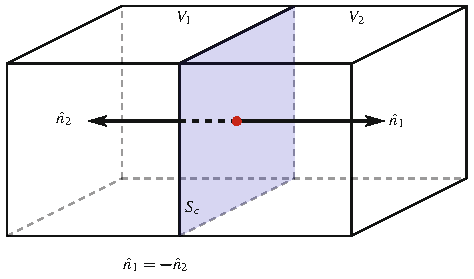
\includegraphics[width=0.562\linewidth]{images/vector/fig-9-6.pdf}
  \caption{共享公共表面 $S_c$ 的两个相邻的立方体积 $V_1$ 和 $V_2$. $V_1$ 的表面 $S_c$ 具有朝外法向量 $\hat{n}_1$，而 $V_2$ 的表面 $S_c$ 具有朝外法向量 $\hat{n}_2$，其中 $\hat{n}_2=-\hat{n}_1$}
  \label{fig:9-6}
\end{figure}

给定一个带曲面 $\partial V$ 的大体积 $V$，如图~\ref{fig:9-7} 所示，它可以被细分为 $N$ 个更小的体积 $V_i$. 此外，这些小体积所有内部表面的通量彼此抵消，
\[
\oint_{\partial V}F\cdot\hat{n}\,dS\approx\sum_{i=1}^{N}\frac{1}{\Delta V_i}\oint_{S_i}F\cdot\hat{n}\,dS\ \Delta V_i=\sum_{i=1}^{N}(\operatorname{div}F)_i\Delta V_i.
\]
当我们取 $N\to\infty$ 且 $|\Delta V_i|\to0$ 的极限时，由于内部表面全部抵消，$\sum V_i\to V$ 且 $\sum\partial V_i\to\partial V$. 所以当我们取极限时，得到下面的等式：
\[
\oint_{\partial V}F\cdot\hat{n}\,dS=\lim_{\substack{N\to\infty\\|\Delta V_i|\to0}}\sum_{i=1}^{N}(\operatorname{div}F)_i\Delta V_i=\iiint_V\operatorname{div}F\,dV,
\]

\begin{figure}[htbp]
  \centering
  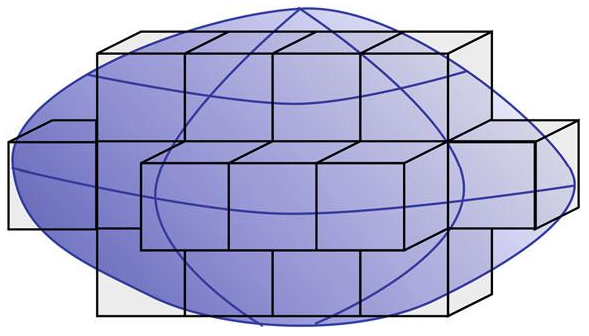
\includegraphics[width=0.815\linewidth]{images/vector/fig-9-7.pdf}
  \caption{被较小的立方体积 $V_i$ 覆盖的不规则形状的体积 $V$. 当 $\Delta V_i\to0$ 时，不规则形状的体积被逼近得越来越好}
  \label{fig:9-7}
\end{figure}

这正是散度定理. 回想 $V$ 的边界是 $\partial V=S$，并把 $F\cdot dS$ 写成 $F\cdot\hat{n}\,dS$，散度定理通常写成
\begin{theorem}[散度定理]\label{thm:9-2}
\[
\oint_{\partial V}F\cdot dS=\iiint_V\operatorname{div}F\,dV.
\]
\end{theorem}

在本节中，我们使用了 $\mathbb{R}^3$ 上用笛卡尔坐标书写的向量场 $F$ 的散度定义，求出了 $\operatorname{div}F$ 的表达式. 但笛卡尔坐标并不是 $\mathbb{R}^3$ 上唯一的坐标系. 第 6.5 节中引入的柱坐标系和球坐标系也是 $\mathbb{R}^3$ 上非常常用的坐标系.

\begin{question}\label{q:9-2}
假设 $F=F_r\hat{e}_r+F_\theta\hat{e}_\theta+F_z\hat{e}_z$ 是关于柱坐标书写的 $\mathbb{R}^3$ 上的向量场. 向量 $\hat{e}_r$ 是 $r$ 增大方向的单位向量，$\hat{e}_\theta$ 是 $\theta$ 增大方向的单位向量，$\hat{e}_z$ 是 $z$ 增大方向的单位向量. 利用图~\ref{fig:6-14} 中所示的柱坐标体积元素和与本节类似的过程，证明
\[
\operatorname{div}F=\frac{1}{r}\frac{\partial(rF_r)}{\partial r}+\frac{1}{r}\frac{\partial F_\theta}{\partial\theta}+\frac{\partial F_z}{\partial z}.
\]
\end{question}

\begin{question}\label{q:9-3}
假设 $F=F_r\hat{e}_r+F_\theta\hat{e}_\theta+F_\varphi\hat{e}_\varphi$ 是关于球坐标书写的 $\mathbb{R}^3$ 上的向量场. 向量 $\hat{e}_r$ 是 $r$ 增大方向的单位向量，$\hat{e}_\theta$ 是 $\theta$ 增大方向的单位向量，$\hat{e}_\varphi$ 是 $\varphi$ 增大方向的单位向量. 利用图~\ref{fig:6-16} 中所示的球坐标体积元素和与本节类似的过程，证明
\[
\operatorname{div}F=\frac{1}{r^2}\frac{\partial(r^2F_r)}{\partial r}+\frac{1}{r\sin\theta}\frac{\partial(\sin\theta\,F_\theta)}{\partial\theta}+\frac{1}{r\sin\theta}\frac{\partial F_\varphi}{\partial\varphi}.
\]
\end{question}

\section{旋度}

给定一个向量场 $F=P\hat{\imath}+Q\hat{\jmath}+R\hat{k}$，在向量微积分课程中，向量场的旋度通常定义为
\[
\operatorname{curl}F=\Bigl(\frac{\partial R}{\partial y}-\frac{\partial Q}{\partial z}\Bigr)\hat{\imath}+\Bigl(\frac{\partial P}{\partial z}-\frac{\partial R}{\partial x}\Bigr)\hat{\jmath}+\Bigl(\frac{\partial Q}{\partial x}-\frac{\partial P}{\partial y}\Bigr)\hat{k}.
\]
常常你还会看到这样的写法：
\[
\operatorname{curl}F=\nabla\times F,
\]
其中 $\nabla$ 就是前面定义的算子
\[
\nabla=\frac{\partial}{\partial x}\hat{\imath}+\frac{\partial}{\partial y}\hat{\jmath}+\frac{\partial}{\partial z}\hat{k},
\]
并且使用了记住两个向量``叉积''$\times$ 的常用记忆辅助手段：
\[
\nabla\times F=\begin{vmatrix}
\hat{\imath}&\hat{\jmath}&\hat{k}\\[2pt]
\dfrac{\partial}{\partial x}&\dfrac{\partial}{\partial y}&\dfrac{\partial}{\partial z}\\[2pt]
P&Q&R
\end{vmatrix}.
\]
重要的是要认识到，$\nabla\times F$ 的这种表述实际上只不过是一种记忆辅助手段，帮助我们重构 $\operatorname{curl}F$ 的公式，假设我们记得如何取 $3\times3$ 矩阵的行列式. 再次，和散度的情况一样，我们将采取稍微不同的方法，以更几何的方式定义旋度，使得 $\operatorname{curl}F$ 的公式和 Stokes 定理都能直接落出来. 然而，在我们真正做出这个定义之前，我们需要理解一些必要的背景材料.

我们从考虑点积的几何意义开始：
\[
v\cdot w=|v|\,|w|\cos\theta,
\]
如图~\ref{fig:9-8} 所示. 如果 $|v|=1$，即 $v$ 是单位向量，那么 $v\cdot w=|w|\cos\theta$，这是 $w$ 指向 $v$ 方向的分量. 现在假设我们想以某种方式度量向量场 $F$ 在某个曲线 $C$ 方向上的``分量''. 我们可以用刚定义的点积来求出它，见图~\ref{fig:9-10}. 之后我们将想要对我们求出的这个``分量''积分.

\begin{figure}[htbp]
  \centering
  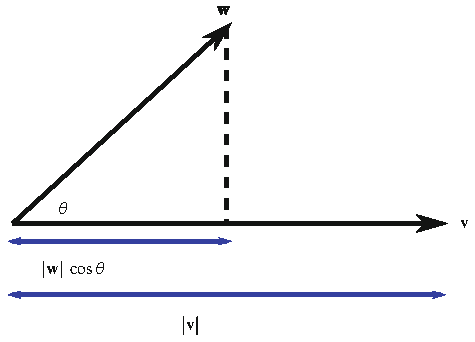
\includegraphics[width=0.563\linewidth]{images/vector/fig-9-8.pdf}
  \caption{点积的几何意义 $v\cdot w=|v|\,|w|\cos\theta$.}
  \label{fig:9-8}
\end{figure}

然而，我们首先需要理解向量场的线积分. 同样，我们假设你上过向量微积分课程，所以我们介绍这些材料时不作太多细节. 不过，我们需要做一个记号的说明以帮助你避免混淆. 我们将围绕闭曲线积分，用 $C$ 表示闭曲线. 这些闭曲线将由弧长参数化，我们用小写字母 $s$ 表示弧长. 我们用大写字母 $S$ 表示边界为曲线 $C$ 的曲面，即 $C=\partial S$. 如果曲线 $C$ 位于一个平面内，我们假定曲面 $S$ 也位于该平面内. 如果是这种情况，那么曲面 $S$ 的单位法向量记为 $\hat{n}$. 为让生活更简单，我们在下文中就假定这种情况.

假设曲线 $C$ 由弧长参数化. 曲线 $C$ 上的点 $s$ 的坐标为 $x=x(s)$、$y=y(s)$、$z=z(s)$，点 $s+\Delta s$ 的坐标为 $x+\Delta x=x(s+\Delta s)$、$y+\Delta y=y(s+\Delta s)$、$z+\Delta z=z(s+\Delta s)$，由此给出
\[
\Delta x=x(s+\Delta s)-x(s),\qquad
\Delta y=y(s+\Delta s)-y(s),\qquad
\Delta z=z(s+\Delta s)-z(s).
\]
令 $\Delta r$ 是从点 $\bigl(x(s),y(s),z(s)\bigr)$ 到点 $\bigl(x(s+\Delta s),y(s+\Delta s),z(s+\Delta s)\bigr)$ 的向量，我们有
\[
\frac{\Delta r}{\Delta s}=\frac{\Delta x}{\Delta s}\hat{\imath}+\frac{\Delta y}{\Delta s}\hat{\jmath}+\frac{\Delta z}{\Delta s}\hat{k}.
\]
我们通过取右边当 $\Delta s\to0$ 时的极限来定义新的向量 $\hat{t}$，这当然也意味着 $\Delta x,\Delta y,\Delta z\to0$：
\[
\hat{t}=\lim_{\Delta s\to0}\Bigl(\frac{\Delta x}{\Delta s}\hat{\imath}+\frac{\Delta y}{\Delta s}\hat{\jmath}+\frac{\Delta z}{\Delta s}\hat{k}\Bigr)=\frac{dx}{ds}\hat{\imath}+\frac{dy}{ds}\hat{\jmath}+\frac{dz}{ds}\hat{k}.
\]

\begin{figure}[htbp]
  \centering
  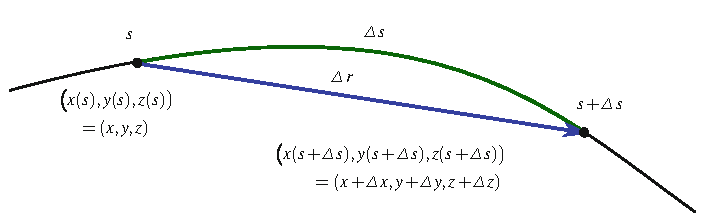
\includegraphics[width=0.840\linewidth]{images/vector/fig-9-9.pdf}
  \caption{曲线的单位切向量 $\hat{t}$ 是 $\Delta r/\Delta s=\frac{\Delta x}{\Delta s}\hat{\imath}+\frac{\Delta y}{\Delta s}\hat{\jmath}+\frac{\Delta z}{\Delta s}\hat{k}$ 的极限}
  \label{fig:9-9}
\end{figure}

从图~\ref{fig:9-9} 可以看出，$\hat{t}$ 是曲线 $C$ 的切向量. 此外，当 $\Delta s\to0$ 时容易看出 $|\Delta r|\to\Delta s$. 因此 $|\hat{t}|=1$，所以 $\hat{t}$ 是曲线 $C$ 的\newterm{unit-tangent-vector}{单位切向量}{unit tangent vector}. 另外，注意形式上我们可以写 $\hat{t}\,ds=\hat{\imath}dx+\hat{\jmath}dy+\hat{k}dz$，我们把它定义为 $ds$.

现在我们转向向量场 $F=P\hat{\imath}+Q\hat{\jmath}+R\hat{k}$ 沿曲线 $C$（由弧长 $s$ 参数化）的线积分. 沿曲线 $C$ 的方向的 $F$ 的分量由 $F\cdot\hat{t}$ 给出，其中 $\hat{t}$ 是 $C$ 的单位切向量. 见图~\ref{fig:9-10} 和图~\ref{fig:9-11}. 假设我们把曲线 $C$ 分成小段，每段长度为 $\Delta s$. 那么每一段上沿 $C$ 方向的 $F$ 的分量可以近似为 $(F\cdot\hat{t})\Delta s$：
\[
(F\cdot\hat{t})\Delta s=\Bigl(P\hat{\imath}+Q\hat{\jmath}+R\hat{k}\Bigr)\cdot\Bigl(\frac{\Delta x}{\Delta s}\hat{\imath}+\frac{\Delta y}{\Delta s}\hat{\jmath}+\frac{\Delta z}{\Delta s}\hat{k}\Bigr)\Delta s
=\Bigl(P\frac{\Delta x}{\Delta s}+Q\frac{\Delta y}{\Delta s}+R\frac{\Delta z}{\Delta s}\Bigr)\Delta s.
\]

\begin{figure}[htbp]
  \centering
  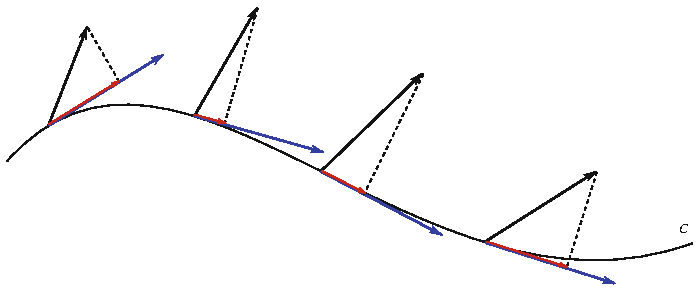
\includegraphics[width=0.958\linewidth]{images/vector/fig-9-10.pdf}
  \caption{向量场 $F$（黑色）定义在曲线 $C$ 上. 我们想知道 $F$ 与 $C$ 相切的那``部分''. 为此我们考虑 $C$ 的单位切向量 $\hat{t}$（蓝色），并求 $F\cdot\hat{t}$（红色），以找出 $F$ 指向 $\hat{t}$ 方向、从而与曲线 $C$ 相切的那``部分''. 我们在曲线 $C$ 的每一点都这样做. 另见图~\ref{fig:9-11}}
  \label{fig:9-10}
\end{figure}

\begin{figure}[htbp]
  \centering
  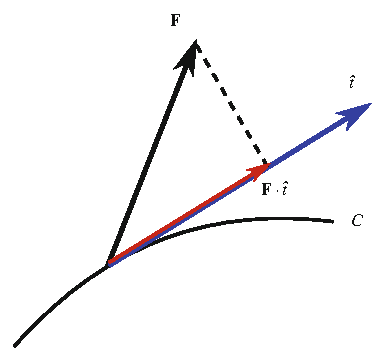
\includegraphics[width=0.452\linewidth]{images/vector/fig-9-11.pdf}
  \caption{图~\ref{fig:9-10} 中一段的放大图. 我们想知道 $F$ 与 $C$ 相切的那``部分''. 为此我们考虑 $C$ 的单位切向量 $\hat{t}$（蓝色），并求 $F\cdot\hat{t}$（红色），以找出 $F$ 指向 $\hat{t}$ 方向、从而与曲线 $C$ 相切的那``部分''}
  \label{fig:9-11}
\end{figure}

所以我们得到
\[
\int_C F\cdot\hat{t}\,ds=\lim_{|\Delta s|\to0}\sum\Bigl(P\frac{\Delta x}{\Delta s}+Q\frac{\Delta y}{\Delta s}+R\frac{\Delta z}{\Delta s}\Bigr)\Delta s.
\]
利用上一段中的记号，积分 $\int_C F\cdot\hat{t}\,ds$ 也可以写成 $\int_C F\cdot ds$.

现在我们知道了沿曲线积分向量场意味着什么，就可以准备定义 $\operatorname{curl}F$ 在点 $(x_0,y_0,z_0)$ 处的值了：
\begin{definition}[旋度的定义]\label{def:9-2-1}
\[
\hat{n}\cdot\operatorname{curl}F=\lim_{|\Delta S|\to0}\frac{1}{\Delta S}\oint_C F\cdot\hat{t}\,ds,
\]
其中 $S$ 是以闭曲线 $C=\partial S$ 为边界的曲面，$\Delta S$ 是该曲面的面积，$\hat{n}$ 是该曲面的单位法向量，$ds$ 中的 $s$ 是无穷小弧长元素，曲面面积 $\Delta S$ 围绕点 $(x_0,y_0,z_0)$ 收缩到零.
\end{definition}

回忆，法向量与曲面 $S$ 所在平面正交，即与之成直角. 曲线 $C$、$F$ 以及 $F$ 沿曲线的分量显示在图~\ref{fig:9-12} 中. 对这个积分积分、除以 $\Delta S$，然后取 $\Delta S\to0$ 的极限，就给出 $\operatorname{curl}F$ 定义右边的值. 本质上，旋度是向量场 $F$ 绕某点无穷小路径的每单位面积的``环流''.

\begin{figure}[htbp]
  \centering
  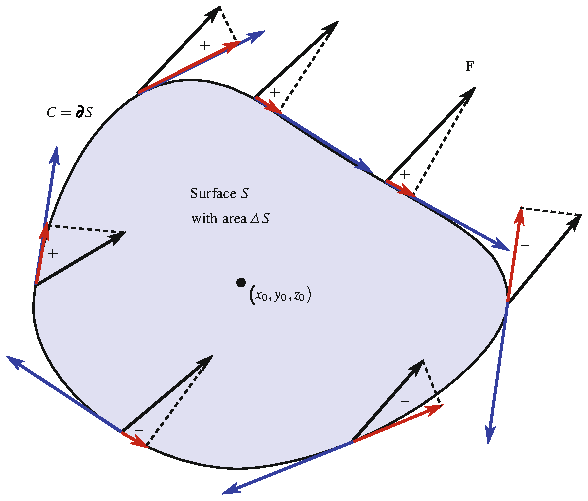
\includegraphics[width=0.720\linewidth]{images/vector/fig-9-12.pdf}
  \caption{图中显示了沿闭曲线 $C$ 的向量场 $F$（黑色）. 图中显示了 $C$ 的单位切向量（蓝色）以及 $F$ 沿 $C$ 的``部分''（红色）. 注意，有时 $F$ 沿 $C$ 的``部分''为正，有时为负}
  \label{fig:9-12}
\end{figure}

\begin{question}\label{q:9-4}
利用图~\ref{fig:9-12} 和如图所示的向量场 $F$，根据积分定义为 $(F\cdot\hat{t})\Delta s$ 之和的极限，估计 $\oint_C F\cdot\hat{t}\,ds$. 换句话说，这个积分是大的还是小的、正的还是负的数，还是接近于零？根据积分的定义解释你的答案.
\end{question}

\begin{question}\label{q:9-5}
画一个像图~\ref{fig:9-12} 那样的图，其中向量场 $F$ 围绕 $(x_0,y_0,z_0)$ 逆时针旋转. 假设 $C$ 的切向量也是逆时针方向的. 积分 $\oint_C F\cdot\hat{t}\,ds$ 是大的还是小的、正的还是负的数，还是接近于零？利用图和积分的定义方式解释为什么. 对顺时针旋转的向量场 $F$ 重复上述过程.
\end{question}

我们想尽力理解这个古怪的定义. 希望最后两个问题已经说明，我们是在试图度量向量场 $F$ 是如何围绕某点``旋转''的. 当我们取 $|\Delta S|\to0$ 的极限时，得到的是点 $(x_0,y_0,z_0)$ 处每单位面积的环流. 但注意定义的左边，$\operatorname{curl}F$ 与曲面 $S$ 的单位法向量 $\hat{n}$ 点积，这告诉我们 $\operatorname{curl}F$ 本身一定是一个向量.

使这个定义有点棘手的问题是，在 $\mathbb{R}^3$ 中，有无数个平面通过点 $(x_0,y_0,z_0)$，因此有无数个可能的曲面 $S$ 及其对应的边界 $\partial S=C$，它们都可以围绕点 $(x_0,y_0,z_0)$ 收缩到面积为零. 也就是说，这本质上就是为什么旋度的定义这么古怪、需要点积的原因. 这个定义必须对通过 $(x_0,y_0,z_0)$ 的每个可能的平面以及该平面内围绕 $(x_0,y_0,z_0)$ 收缩到面积为零的每个可能的曲面 $S$ 都成立. 左边 $\hat{n}$（曲面 $S$ 的单位法向量）与 $\operatorname{curl}F$ 的点积，对应于（或者说补偿了）在右边选择某个放置曲面 $S$ 和曲线 $C$ 的特定平面.

让我们花几分钟更深入地探索一下. 考虑图~\ref{fig:9-13}，其中显示了围绕点 $(x_0,y_0,z_0)$ 的、边界为 $\partial S=C$ 的曲面 $S$. 沿 $C$ 的几个点处，曲线 $C$ 的单位切向量 $\hat{t}$ 用蓝色显示，在这些相同点处向量场 $F$ 用黑色显示. 每个场向量在 $\hat{t}$ 方向的分量显示为红色的 $F\cdot\hat{t}$，并且也标出了它的符号：如果 $F\cdot\hat{t}$ 指向 $\hat{t}$ 方向则为正，如果 $F\cdot\hat{t}$ 指向 $-\hat{t}$ 方向则为负. 我们把向量场 $F$ 中的所有向量都画成互相平行，以表明点 $(x_0,y_0,z_0)$ 周围没有环流发生. 这意味着正的 $F\cdot\hat{t}$ 的``量''与负的 $F\cdot\hat{t}$ 的``量''完全相同，导致 $\oint_C F\cdot\hat{t}\,ds=0$. 图中还显示了在点 $(x_0,y_0,z_0)$ 处画出的曲面 $S$ 的单位法向量 $\hat{n}$. 我们画 $\hat{n}$ 时让它相对于单位切向量 $\hat{t}$（蓝色）遵循右手法则. 我们这样做只是为了在不同曲面之间标准化 $F\cdot\hat{t}$ 的正负. 利用我们的旋度定义，我们有
\[
\hat{n}\cdot\operatorname{curl}F=\lim_{|\Delta S|\to0}\frac{1}{\Delta S}\oint_C F\cdot\hat{t}\,ds=0.
\]

\begin{figure}[htbp]
  \centering
  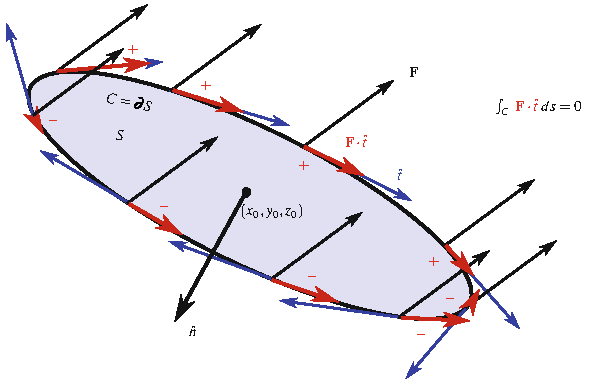
\includegraphics[width=0.720\linewidth]{images/vector/fig-9-13.pdf}
  \caption{$\hat{n}\cdot\operatorname{curl}F=0$ 的示意图. 我们画出了 $\operatorname{curl}F$ 定义中出现的所有分量，但向量 $\operatorname{curl}F$ 本身除外}
  \label{fig:9-13}
\end{figure}

所以，虽然我们可能实际上还不知道向量 $\operatorname{curl}F$ 是什么，但我们知道它必须垂直于 $\hat{n}$，因为 $\hat{n}\cdot\operatorname{curl}F=0$.

现在考虑图~\ref{fig:9-14}，其中几乎所有内容都与上一图相同，只是这次向量场 $F$ 的向量在某种意义上围绕点 $(x_0,y_0,z_0)$ 旋转. 注意现在所有的 $F\cdot\hat{t}$ 都指向与 $\hat{t}$ 相同的方向，因此都是正的. 这意味着
\[
\hat{n}\cdot\operatorname{curl}F=\lim_{|\Delta S|\to0}\frac{1}{\Delta S}\oint_C F\cdot\hat{t}\,ds>0.
\]

\begin{figure}[htbp]
  \centering
  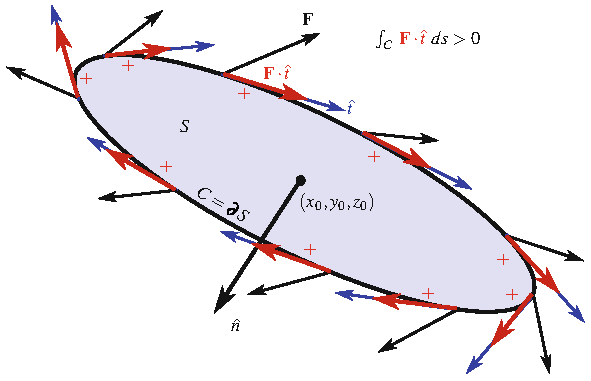
\includegraphics[width=0.700\linewidth]{images/vector/fig-9-14.pdf}
  \caption{$\hat{n}\cdot\operatorname{curl}F>0$ 的示意图. 同样我们画出了 $\operatorname{curl}F$ 定义中出现的所有分量，但向量 $\operatorname{curl}F$ 本身除外}
  \label{fig:9-14}
\end{figure}

所以，再次地，虽然我们可能实际上还不知道向量 $\operatorname{curl}F$ 是什么，但我们知道它与 $\hat{n}$ 点积时为正.

所以，实际求出向量 $\operatorname{curl}F$ 是什么，需要我们仔细地选择曲面及其对应的法向量. 显然，任何向量，包括向量 $\operatorname{curl}F$，都是欧几里得单位向量 $\hat{\imath}$、$\hat{\jmath}$ 和 $\hat{k}$ 的线性组合. 为了求出 $\operatorname{curl}F$ 中沿 $\hat{\imath}$ 方向的分量，我们需要求 $\operatorname{curl}F\cdot\hat{\imath}$. 类似地，为了求出 $\operatorname{curl}F$ 中沿 $\hat{\jmath}$ 方向的分量，我们需要求 $\operatorname{curl}F\cdot\hat{\jmath}$，为了求出 $\operatorname{curl}F$ 中沿 $\hat{k}$ 方向的分量，我们需要求 $\operatorname{curl}F\cdot\hat{k}$. 所以通过选择平行于 $yz$ 平面的 $S$，我们得到 $\hat{n}=\hat{\imath}$，这让我们能求出 $\operatorname{curl}F$ 的 $\hat{\imath}$ 项. 类似地，选择平行于 $xz$ 平面的 $S$ 给出 $\hat{n}=\hat{\jmath}$，这让我们能求出 $\operatorname{curl}F$ 的 $\hat{\jmath}$ 项，而选择平行于 $xy$ 平面的 $S$ 给出 $\hat{n}=\hat{k}$，这让我们能求出 $\operatorname{curl}F$ 的 $\hat{k}$ 项.

我们从选择平行于 $xy$ 平面（单位法向量为 $\hat{k}$）的平面内、围绕点 $(x_0,y_0,z_0)$ 的一条路径开始. 任何路径都可以，为简单起见我们选择图~\ref{fig:9-15} 中所示的正方形路径. 从上方俯视这条路径，我们可以把曲线的上、下、左、右边标为 $C_T$、$C_B$、$C_L$ 和 $C_R$，如图所示.

\begin{figure}[htbp]
  \centering
  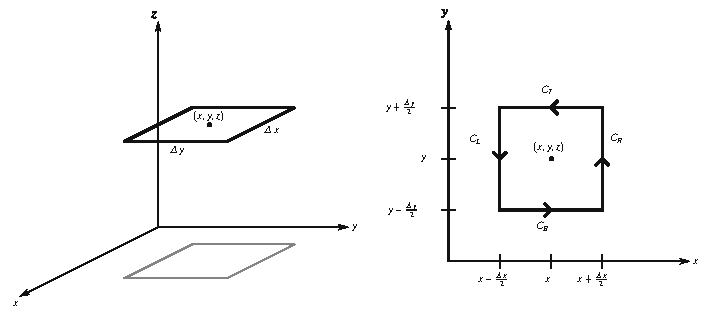
\includegraphics[width=0.960\linewidth]{images/vector/fig-9-15.pdf}
  \caption{围绕点 $(x,y,z)$ 的正方形曲线. 这条曲线位于平行于 $xy$ 平面的平面内（左），该平面具有单位法向量 $\hat{k}$. 从上方俯视同一条正方形曲线（右）. 这条正方形曲线由四条线段 $C_T$、$C_B$、$C_L$ 和 $C_R$ 组成}
  \label{fig:9-15}
\end{figure}

沿 $C_B$，单位切向量是 $\hat{t}=\hat{\imath}$，它给出 $F\cdot\hat{t}=F\cdot\hat{\imath}=P$. 所以我们有
\[
\oint_{C_B}F\cdot\hat{t}\,ds=\int_{C_B}P\,ds\approx P\Bigl(x_0,y_0-\frac{\Delta y}{2},z_0\Bigr)\Delta x.
\]
沿 $C_T$，单位切向量是 $\hat{t}=-\hat{\imath}$，它给出 $F\cdot\hat{t}=F\cdot(-\hat{\imath})=-P$. 所以我们有
\[
\oint_{C_T}F\cdot\hat{t}\,ds=\int_{C_T}-P\,ds\approx -P\Bigl(x_0,y_0+\frac{\Delta y}{2},z_0\Bigr)\Delta x.
\]
合在一起有
\begin{align*}
\oint_{C_T+C_B}F\cdot\hat{t}\,ds=-\frac{P\bigl(x_0,y_0+\frac{\Delta y}{2},z_0\bigr)-P\bigl(x_0,y_0-\frac{\Delta y}{2},z_0\bigr)}{\Delta y}\Delta x\Delta y, \\
\Rightarrow\quad\lim_{|\Delta S|\to0}\frac{1}{\Delta S}\oint_{C_T+C_B}F\cdot\hat{t}\,ds
=\lim_{\Delta y\to0}-\frac{P\bigl(x_0,y_0+\frac{\Delta y}{2},z_0\bigr)-P\bigl(x_0,y_0-\frac{\Delta y}{2},z_0\bigr)}{\Delta y}
=-\frac{\partial P}{\partial y}.
\end{align*}
沿 $C_R$，单位切向量是 $\hat{t}=\hat{\jmath}$，它给出 $F\cdot\hat{t}=F\cdot\hat{\jmath}=Q$. 所以我们有
\[
\oint_{C_R}F\cdot\hat{t}\,ds=\int_{C_R}Q\,ds\approx Q\Bigl(x_0+\frac{\Delta x}{2},y_0,z_0\Bigr)\Delta y.
\]
沿 $C_L$，单位切向量是 $\hat{t}=-\hat{\jmath}$，它给出 $F\cdot\hat{t}=F\cdot(-\hat{\jmath})=-Q$. 所以我们有
\[
\oint_{C_L}F\cdot\hat{t}\,ds=\int_{C_L}-Q\,ds\approx -Q\Bigl(x_0-\frac{\Delta x}{2},y_0,z_0\Bigr)\Delta y.
\]
合在一起有
\begin{align*}
\oint_{C_R+C_L}F\cdot\hat{t}\,ds=\frac{Q\bigl(x_0+\frac{\Delta x}{2},y_0,z_0\bigr)-Q\bigl(x_0-\frac{\Delta x}{2},y_0,z_0\bigr)}{\Delta x}\Delta x\Delta y, \\
\Rightarrow\quad\lim_{|\Delta S|\to0}\frac{1}{\Delta S}\oint_{C_R+C_L}F\cdot\hat{t}\,ds
=\lim_{\Delta x\to0}\frac{Q\bigl(x_0+\frac{\Delta x}{2},y_0,z_0\bigr)-Q\bigl(x_0-\frac{\Delta x}{2},y_0,z_0\bigr)}{\Delta x}
=\frac{\partial Q}{\partial x}.
\end{align*}
由于 $xy$ 平面的法向量是 $\hat{k}$，我们得到
\[
\hat{k}\cdot\operatorname{curl}F=\lim_{|\Delta S|\to0}\frac{1}{\Delta S}\oint_{C_L+C_R+C_B+C_T}F\cdot\hat{t}\,ds=\frac{\partial Q}{\partial x}-\frac{\partial P}{\partial y}.
\]
所以这就是 $\operatorname{curl}F$ 在 $\hat{k}$ 方向的分量.

\begin{question}\label{q:9-6}
重复上面的计算，求出 $\operatorname{curl}F$ 在 $\hat{\imath}$ 方向的分量是 $\frac{\partial R}{\partial y}-\frac{\partial Q}{\partial z}$，$\operatorname{curl}F$ 在 $\hat{\jmath}$ 方向的分量是 $\frac{\partial P}{\partial z}-\frac{\partial R}{\partial x}$.
\end{question}

因此，从我们的旋度定义出发，我们推导出了下面的公式：
\begin{theorem}[旋度的计算公式（笛卡尔坐标）]\label{thm:9-3}
\[
\operatorname{curl}F=\Bigl(\frac{\partial R}{\partial y}-\frac{\partial Q}{\partial z}\Bigr)\hat{\imath}+\Bigl(\frac{\partial P}{\partial z}-\frac{\partial R}{\partial x}\Bigr)\hat{\jmath}+\Bigl(\frac{\partial Q}{\partial x}-\frac{\partial P}{\partial y}\Bigr)\hat{k}.
\]
\end{theorem}

Stokes 定理基本上从这一定义中落出来. 我们将（以非常不严格的方式）``推导''这个定理. 给定任何边界为闭曲线 $C$ 的曲面 $S$（不一定在平面内），我们可以把它分成带边界 $C_i$ 的子曲面 $S_i$，如图~\ref{fig:9-16} 所示.

\begin{figure}[htbp]
  \centering
  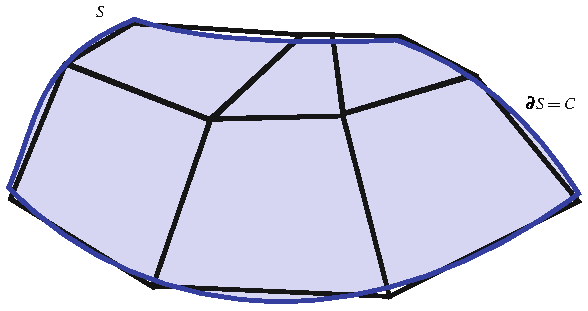
\includegraphics[width=0.696\linewidth]{images/vector/fig-9-16.pdf}
  \caption{边界为闭曲线 $\partial S=C$ 的曲面 $S$ 被较小的曲面 $S_i$ 覆盖. 当 $\Delta S_i\to0$ 时，曲面 $S$ 被逼近得越来越好}
  \label{fig:9-16}
\end{figure}

通过与上一节类似的推理，如果两个 $C_i$ 共享一条边，我们有
\[
\int_A F\cdot\hat{t}\,ds=-\int_B F\cdot\hat{t}\,ds
\]
所以这些项抵消，见图~\ref{fig:9-17}. 因此
\begin{align*}
\oint_{\partial S=C}F\cdot\hat{t}\,ds=\lim_{\substack{N\to\infty\\|\Delta S_i|\to0}}\sum_{i=0}^{N}\oint_{C_i}F\cdot\hat{t}\,ds
=\lim_{\substack{N\to\infty\\|\Delta S_i|\to0}}\sum_{i=0}^{N}\frac{1}{\Delta S_i}\oint_{C_i}F\cdot\hat{t}\,ds\ \Delta S_i \\
=\lim_{\substack{N\to\infty\\|\Delta S_i|\to0}}\sum_{i=0}^{N}\Bigl(\lim_{|\Delta S_i|\to0}\frac{1}{\Delta S_i}\oint_{C_i}F\cdot\hat{t}\,ds\Bigr)\Delta S_i
=\lim_{\substack{N\to\infty\\|\Delta S_i|\to0}}\sum_{i=0}^{N}\bigl(\hat{n}_i\cdot\operatorname{curl}F\bigr)_i\Delta S_i \\
=\iint_S\bigl(\hat{n}\cdot\operatorname{curl}F\bigr)\,dS,
\end{align*}

\begin{figure}[htbp]
  \centering
  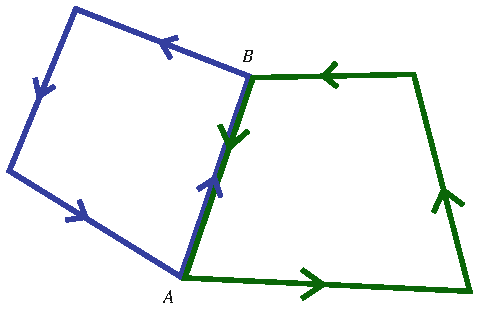
\includegraphics[width=0.568\linewidth]{images/vector/fig-9-17.pdf}
  \caption{共享边界 $C_i$（即点 $A$ 与 $B$ 之间的线段）的两个相邻的子曲面}
  \label{fig:9-17}
\end{figure}

这正是 Stokes 定理：
\begin{theorem}[Stokes 定理]\label{thm:9-4}
\[
\oint_{\partial S}F\cdot\hat{t}\,ds=\iint_S\bigl(\hat{n}\cdot\operatorname{curl}F\bigr)\,dS.
\]
\end{theorem}

写 Stokes 定理的另一种方式是
\[
\oint_{\partial S}F\cdot ds=\iint_S\operatorname{curl}F\cdot dS.
\]

在本节中，我们使用了 $\mathbb{R}^3$ 上用笛卡尔坐标书写的向量场 $F$ 的旋度定义，求出了 $\operatorname{curl}F$ 的表达式. 但当然，第 6.5 节中引入的柱坐标系和球坐标系也是 $\mathbb{R}^3$ 上非常常用的坐标系.

\begin{question}\label{q:9-7}
假设 $F=F_r\hat{e}_r+F_\theta\hat{e}_\theta+F_z\hat{e}_z$ 是关于柱坐标书写的 $\mathbb{R}^3$ 上的向量场. 向量 $\hat{e}_r$ 是 $r$ 增大方向的单位向量，$\hat{e}_\theta$ 是 $\theta$ 增大方向的单位向量，$\hat{e}_z$ 是 $z$ 增大方向的单位向量. 利用与图~\ref{fig:6-14} 中所示柱坐标体积元素的每个面对应的边类似的曲线，以及和本节类似的过程，证明
\[
\operatorname{curl}F=(\operatorname{curl}F)_r\hat{e}_r+(\operatorname{curl}F)_\theta\hat{e}_\theta+(\operatorname{curl}F)_z\hat{e}_z,
\]
其中
\[
(\operatorname{curl}F)_r=\frac{1}{r}\frac{\partial F_z}{\partial\theta}-\frac{\partial F_\theta}{\partial z},\qquad
(\operatorname{curl}F)_\theta=\frac{\partial F_r}{\partial z}-\frac{\partial F_z}{\partial r},\qquad
(\operatorname{curl}F)_z=\frac{1}{r}\frac{\partial(rF_\theta)}{\partial r}-\frac{1}{r}\frac{\partial F_r}{\partial\theta}.
\]
\end{question}

\begin{question}\label{q:9-8}
假设 $F=F_r\hat{e}_r+F_\theta\hat{e}_\theta+F_\varphi\hat{e}_\varphi$ 是关于球坐标书写的 $\mathbb{R}^3$ 上的向量场. 向量 $\hat{e}_r$ 是 $r$ 增大方向的单位向量，$\hat{e}_\theta$ 是 $\theta$ 增大方向的单位向量，$\hat{e}_\varphi$ 是 $\varphi$ 增大方向的单位向量. 利用与图~\ref{fig:6-16} 中所示球坐标体积元素的每个面对应的边类似的曲线，以及和本节类似的过程，证明
\[
\operatorname{curl}F=(\operatorname{curl}F)_r\hat{e}_r+(\operatorname{curl}F)_\theta\hat{e}_\theta+(\operatorname{curl}F)_\varphi\hat{e}_\varphi,
\]
其中
\begin{align*}
(\operatorname{curl}F)_r=\frac{1}{r\sin\theta}\frac{\partial(\sin\theta\,F_\varphi)}{\partial\theta}-\frac{1}{r\sin\theta}\frac{\partial F_\theta}{\partial\varphi},\qquad
(\operatorname{curl}F)_\theta=\frac{1}{r\sin\theta}\frac{\partial F_r}{\partial\varphi}-\frac{1}{r}\frac{\partial(rF_\varphi)}{\partial r}, \\
(\operatorname{curl}F)_\varphi=\frac{1}{r}\frac{\partial(rF_\theta)}{\partial r}-\frac{1}{r}\frac{\partial F_r}{\partial\theta}.
\end{align*}
\end{question}

\section{梯度}

梯度比散度或旋度更直截了当. 在向量微积分中，函数 $f:\mathbb{R}^3\to\mathbb{R}$ 的梯度通常简单地定义为向量场
\[
\operatorname{grad}f=\frac{\partial f}{\partial x}\hat{\imath}+\frac{\partial f}{\partial y}\hat{\jmath}+\frac{\partial f}{\partial z}\hat{k}.
\]
一般 $\operatorname{grad}f$ 写成 $\nabla f$. 此外，在向量微积分中我们还学到，函数 $f$ 沿单位长度向量 $u$ 方向的方向导数可以写成 $D_uf=\nabla f\cdot u$，或者写成 $u[f]=\nabla f\cdot u$.

我们基本上是反过来定义函数 $f$ 的梯度：把它定义为与单位长度向量 $u$ 点积后给出 $f$ 沿方向 $u$ 的方向导数的那个向量场：
\begin{definition}[梯度的定义]\label{def:9-3-1}
\[
\operatorname{grad}f\cdot u=u[f].
\]
\end{definition}

在第 2.3 节中我们基本上证明了，在使用笛卡尔坐标系时可以写成
\begin{theorem}[梯度的计算公式（笛卡尔坐标）]\label{thm:9-5}
\[
\operatorname{grad}f=\frac{\partial f}{\partial x}\hat{\imath}+\frac{\partial f}{\partial y}\hat{\jmath}+\frac{\partial f}{\partial z}\hat{k}.
\]
\end{theorem}
因此我们看到，通常的向量微积分定义与我们的定义一致. 当然，在这一点上你应该看到 $f$ 的梯度 $\operatorname{grad}f$ 与 1-形式 $df$ 之间的相似之处.

我们在上一节已经讨论了向量场沿曲线的积分是什么. 向量场 $F$ 沿曲线 $C$ 的积分由 $\int_C F\cdot\hat{t}\,ds$ 给出，其中 $\hat{t}$ 是沿曲线 $C$ 的单位切向量，曲线由弧长 $s$ 参数化. 把曲线写成 $C=c(s)=\bigl(x(s),y(s),z(s)\bigr)$，那么我们有
\[
c'(s)=\Bigl(\frac{dx}{ds},\frac{dy}{ds},\frac{dz}{ds}\Bigr)=\frac{dx}{ds}\hat{\imath}+\frac{dy}{ds}\hat{\jmath}+\frac{dz}{ds}\hat{k},
\]
这显然是曲线 $c(s)$ 的切线. 另外，与上面类似的方式，我们可以形式上写 $c'(s)\,ds=\hat{\imath}dx+\hat{\jmath}dy+\hat{k}dz$ 并把它定义为 $ds$. 假设我们令 $F=\operatorname{grad}f$，那么 $\operatorname{grad}f$ 沿曲线 $c(s)$ 从 $c(a)$ 到 $c(b)$（其中 $a,b\in\mathbb{R}$ 且 $a\leq b$）的积分将是
\[
\begin{aligned}
\int_C\operatorname{grad}f\cdot c'(s)\,ds
&=\int_a^b\Bigl(\frac{\partial f}{\partial x}\hat{\imath}+\frac{\partial f}{\partial y}\hat{\jmath}+\frac{\partial f}{\partial z}\hat{k}\Bigr)\cdot\Bigl(\frac{dx}{ds}\hat{\imath}+\frac{dy}{ds}\hat{\jmath}+\frac{dz}{ds}\hat{k}\Bigr)\,ds\\
&=\int_a^b\Bigl(\frac{\partial f}{\partial x}\frac{dx}{ds}+\frac{\partial f}{\partial y}\frac{dy}{ds}+\frac{\partial f}{\partial z}\frac{dz}{ds}\Bigr)\,ds\\
&=\int_a^b\frac{d}{ds}f\bigl(c(s)\bigr)\,ds\\
&=f\bigl(c(b)\bigr)-f\bigl(c(a)\bigr).
\end{aligned}
\]
倒数第二个等式来自链式法则，最后一个等式来自微积分基本定理. 把 $c'(s)\,ds$ 写成 $ds$，就得到线积分基本定理：
\begin{theorem}[线积分基本定理]\label{thm:9-6}
\[
\int_C\operatorname{grad}f\cdot ds=f\bigl(c(b)\bigr)-f\bigl(c(a)\bigr).
\]
\end{theorem}

在柱坐标中，类似的论证会给出
\[
\operatorname{grad}f=\frac{\partial f}{\partial r}\hat{e}_r+\frac{1}{r}\frac{\partial f}{\partial\theta}\hat{e}_\theta+\frac{\partial f}{\partial z}\hat{e}_z,
\]
其中 $\hat{e}_r$ 是 $r$ 增大方向的单位向量，$\hat{e}_\theta$ 是 $\theta$ 增大方向的单位向量，$\hat{e}_z$ 是 $z$ 增大方向的单位向量. 在球坐标中我们有
\[
\operatorname{grad}f=\frac{\partial f}{\partial r}\hat{e}_r+\frac{1}{r}\frac{\partial f}{\partial\theta}\hat{e}_\theta+\frac{1}{r\sin\theta}\frac{\partial f}{\partial\varphi}\hat{e}_\varphi,
\]
其中当然 $\hat{e}_r$ 是 $r$ 增大方向的单位向量，$\hat{e}_\theta$ 是 $\theta$ 增大方向的单位向量，$\hat{e}_\varphi$ 是 $\varphi$ 增大方向的单位向量.

\begin{question}\label{q:9-9}
函数 $f$ 的\newterm{laplacian}{拉普拉斯算子}{Laplacian}定义为 $\operatorname{div}(\operatorname{grad}f)=\nabla\cdot(\nabla f)=\nabla\cdot\nabla f$. 有时这写成 $\nabla^2f$ 或 $\Delta f$. 求 $f$ 在笛卡尔坐标、柱坐标和球坐标下的拉普拉斯算子.
\end{question}

\section{上下指标、升号与降号}

在继续之前，现在是引入一种特定记号约定的好时机. 这种记号约定对后续内容将很有用. 到目前为止，在这本书中我们一直在努力解释数学概念，因此主要使用数学记号. 然而，随着我们走向许多其他例子和主题，物理学中通常使用的记号将很有用.

不同的记号各有其优缺点，而微分几何就是数学中记号负担很重的领域之一. 数学记号擅长理解理论、理解数学对象实际上是什么、理解数学对象所在的空间，以及理解底层的数学运算和作用. 物理学记号通常更适合进行计算和演算，尽管这种记号可能会掩盖计算底下的数学实质. 要成为一个好的数学家或物理学家，你真的需要对这两种记号都感到自如.

首先我们引入 \newterm{einstein-summation}{Einstein 求和记号}{Einstein summation notation}. 简而言之，Einstein 求和记号的要点是：当你看到重复出现的上下指标时就要求和. 也就是说，如果你看到像
\[
a^ie_i
\]
这样的东西，它实际上表示
\[
\sum_i a^ie_i.
\]
类似地，
\[
a_ie^i\equiv\sum_i a_ie^i.
\]
据说 Einstein 曾经打趣说，求和记号是他对数学的伟大贡献！求和记号在张量微积分中被广泛使用，我们将在附录 A 中引入张量微积分. 暂不讨论这个表达式的含义，考虑
\[
T^{ijk}_{lm}\Lambda^{l}_{jk}.
\]
用 Einstein 求和记号，这实际上表示
\[
\sum_j\sum_k\sum_l T^{ijk}_{lm}\Lambda^{l}_{jk}.
\]
正如你所看到的，每当下指标和上指标重复出现时，我们就对该指标求和. 由于同时存在成对出现的上指标和下指标 $j$、$k$ 和 $l$，我们对 $j$、$k$ 和 $l$ 求和.

考虑向量空间 $V=\operatorname{span}\{e_1,e_2,e_3\}$. $V$ 的元素可以借助系数用基向量 $e_1,e_2,e_3$ 写出. 也就是说，$v\in V$ 可以写成
\[
v=v^1e_1+v^2e_2+v^3e_3=\begin{bmatrix}v^1\\v^2\\v^3\end{bmatrix}=v^ie_i,
\]
其中向量系数 $v^1,v^2,v^3$ 是实数. 注意向量系数用上指标书写. 和往常一样，我们继续把向量看成列矩阵.

$V$ 的对偶空间是 $V^*=\operatorname{Span}\{e^{1*},e^{2*},e^{3*}\}$，其中 $e^{1*},e^{2*},e^{3*}$ 只是 $e_1,e_2,e_3$ 的对偶元素. 也就是说，我们有
\[
\langle e^{i*},e_j\rangle=\delta_{ij}=\begin{cases}1,&i=j,\\0,&i\neq j.\end{cases}
\]
为了从现在起与 Einstein 求和记号保持一致，我们将用上指标书写对偶基元素 $e^1,e^2,e^3$. 也就是说，$e^{1*}\equiv e^1$、$e^{2*}\equiv e^2$、$e^{3*}\equiv e^3$，所以 $\langle e^i,e_j\rangle=e^i(e_j)=\delta^i_j$. 有时你会看到克罗内克 δ 函数写成 $\delta^i_j$，以与 Einstein 求和记号保持一致. $V^*=\operatorname{Span}\{e^1,e^2,e^3\}$ 的元素（有时称为余向量）写成
\[
\alpha=\alpha_1e^1+\alpha_2e^2+\alpha_3e^3=[\alpha_1,\alpha_2,\alpha_3]=\alpha_ie^i,
\]
其中余向量系数 $\alpha_1,\alpha_2,\alpha_3$ 是实数. 再次注意，余向量系数用下指标书写. 和往常一样，我们继续把余向量看成行矩阵. 所以
\[
\begin{aligned}
\langle\alpha,v\rangle=\alpha(v)&=(\alpha_1e^1+\alpha_2e^2+\alpha_3e^3)(v^1e_1+v^2e_2+v^3e_3)\\
&=\alpha_1e^1(v^1e_1+v^2e_2+v^3e_3)+\alpha_2e^2(v^1e_1+v^2e_2+v^3e_3)\\
&\quad+\alpha_3e^3(v^1e_1+v^2e_2+v^3e_3)\\
&=\alpha_1v^1e^1(e_1)+\alpha_1v^2e^1(e_2)+\alpha_1v^3e^1(e_3)\\
&\quad+\alpha_2v^1e^2(e_1)+\alpha_2v^2e^2(e_2)+\alpha_2v^3e^2(e_3)\\
&\quad+\alpha_3v^1e^3(e_1)+\alpha_3v^2e^3(e_2)+\alpha_3v^3e^3(e_3)\\
&=\alpha_1v^1+\alpha_2v^2+\alpha_3v^3.
\end{aligned}
\]
多么凌乱的计算，如果你有比三个多很多的基元素，你不会想这样做，尽管模式当然很清楚. 用传统求和记号做同样的计算是
\[
\begin{aligned}
\langle\alpha,v\rangle=\alpha(v)&=\Bigl(\sum_{i=1}^{3}\alpha_ie^i\Bigr)\Bigl(\sum_{j=1}^{3}v^je_j\Bigr)=\sum_{i=1}^{3}\alpha_ie^i\Bigl(\sum_{j=1}^{3}v^je_j\Bigr)\\
&=\sum_{i=1}^{3}\sum_{j=1}^{3}\alpha_iv^je^i(e_j)=\sum_{i=1}^{3}\alpha_iv^i.\qquad(\text{只有 }j=i\text{ 的项保留下来})
\end{aligned}
\]
最后我们用 Einstein 求和记号做同样的计算：
\[
\begin{aligned}
\langle\alpha,v\rangle=\alpha(v)&=(\alpha_ie^i)(v^je_j)=\alpha_ie^i(v^je_j)\\
&=\alpha_iv^je^i(e_j)=\alpha_iv^i.\qquad(\text{只有 }j=i\text{ 的项保留下来})
\end{aligned}
\]
一旦你对 Einstein 求和记号感到自如，你的手就不用动那么多了.

现在，让我们在微分形式的语境下看看这一切. 目前我们假设 $M=\mathbb{R}^3$. 我们将 $M$ 的笛卡尔坐标函数写成 $x^1,x^2,x^3$，用上指标而不是下指标. 数学家倾向于对坐标函数使用下指标，事实上到目前为止我们正是这样做的，但通过用上指标书写坐标函数，Einstein 求和记号就能漂亮地工作. 所以，在点 $p\in M$ 处，切空间由
\[
T_p\mathbb{R}^3=\operatorname{span}\Bigl\{\left.\frac{\partial}{\partial x^1}\right|_p,\left.\frac{\partial}{\partial x^2}\right|_p,\left.\frac{\partial}{\partial x^3}\right|_p\Bigr\}
=\operatorname{span}\Bigl\{\frac{\partial}{\partial x^1},\frac{\partial}{\partial x^2},\frac{\partial}{\partial x^3}\Bigr\}
\]
给出，其中第二行在记号中省略了基点. 点 $p\in M$ 处的余切空间由
\[
T_p^*\mathbb{R}^3=\operatorname{Span}\Bigl\{\left.dx^1\right|_p,\left.dx^2\right|_p,\left.dx^3\right|_p\Bigr\}
=\operatorname{Span}\{dx^1,dx^2,dx^3\}
\]
给出. 显然我们可以把 $dx^i$ 中的指标看成上指标. 按照惯例，我们把 $\frac{\partial}{\partial x^i}$ 中的指标看成下指标，因为它位于表达式的``分母''中. 因此 $v\in T_p\mathbb{R}^3$ 的元素写成
\[
v=v^1\frac{\partial}{\partial x^1}+v^2\frac{\partial}{\partial x^2}+v^3\frac{\partial}{\partial x^3}=v^i\frac{\partial}{\partial x^i},
\]
其中 $v^1,v^2,v^3$ 是实数. 再次地，向量的系数用上指标书写. $\alpha\in T_p^*\mathbb{R}^3$ 的元素写成
\[
\alpha=\alpha_1dx^1+\alpha_2dx^2+\alpha_3dx^3=\alpha_idx^i,
\]
其中 $\alpha_1,\alpha_2,\alpha_3$ 是实数. 正如我们看到的，余向量，即微分形式，其系数用下指标书写.

总之，向量基元素用下指标书写，向量分量用上指标书写. 余向量（微分形式）基元素用上指标书写，余向量（微分形式）分量用下指标书写.

现在我们引入所谓的\newterm{musical-isomorphism}{音乐同构}{musical isomorphism}. 实际上，音乐同构依赖于一种称为\newterm{metric}{度规}{metric}的东西. 非常粗略地，你可以把度规想成允许你测量两点之间距离的东西. 我们将在引入张量之后讨论欧几里得度规，但本质上它就是我们熟悉的 $\mathbb{R}^n$ 上通常的距离函数. 然而，现在我们还不会那么数学严格，而是给出一个不显式依赖度规的音乐同构的``定义''. 你只要记住，目前我们算是把一些数学理论扫到地毯下面了.

音乐同构之所以称为``音乐''的，是因为所用的记号——\newterm{flat}{降号}{flat} $\flat$ 和\newterm{sharp}{升号}{sharp} $\sharp$. 如果你唱过歌或演奏过乐器，你就知道 $\flat$ 告诉你把音符的音高降低，而 $\sharp$ 告诉你把音符的音高升高. 类似地，$\flat$ 同构被称为``降低指标''，而 $\sharp$ 同构被称为``升高指标''.

$\flat$ 同构由
\[
\flat:T_pM\longrightarrow T_p^*M,\qquad v^i\frac{\partial}{\partial x^i}\longmapsto v_idx^i,\quad\text{其中 }v_i=v^i
\]
给出. 这种映射的写法是 $v^{\flat}$，就像乐谱中降号的写法一样，所以我们写
\[
v^{\flat}=\Bigl(v^i\frac{\partial}{\partial x^i}\Bigr)^{\flat}\equiv v_idx^i,
\]
其中 $v_i=v^i$. 例如我们有
\[
\Bigl(7\frac{\partial}{\partial x^1}+3\frac{\partial}{\partial x^2}-6\frac{\partial}{\partial x^3}\Bigr)^{\flat}=7dx^1+3dx^2-6dx^3.
\]
注意正在发生的事情：我们把一个向量（其分量用上指标书写）变成一个 1-形式（其分量用下指标书写），所以我们是在``降低''指标，这就解释了使用 $\flat$ 符号的原因.

$\sharp$ 同构由
\[
\sharp:T_p^*M\longrightarrow T_pM,\qquad \alpha_idx^i\longmapsto\alpha^i\frac{\partial}{\partial x^i},\quad\text{其中 }\alpha^i=\alpha_i
\]
给出. 同样，这种映射的写法是 $\alpha^{\sharp}$，就像乐谱中升号的写法一样，所以我们写
\[
\alpha^{\sharp}=\Bigl(\alpha_idx^i\Bigr)^{\sharp}\equiv\alpha^i\frac{\partial}{\partial x^i},
\]
其中 $\alpha^i=\alpha_i$. 例如我们有
\[
\bigl(3dx^1-9dx^2+8dx^3\bigr)^{\sharp}=3\frac{\partial}{\partial x^1}-9\frac{\partial}{\partial x^2}+8\frac{\partial}{\partial x^3}.
\]
我们正在把一个微分 1-形式（或余向量）（其分量用下指标书写）变成一个向量（其分量用上指标书写），所以我们是在``升高''指标，这就解释了使用 $\sharp$ 符号的原因.

你应该注意，降号和升号算子的这些``定义''只有在用笛卡尔坐标书写我们的向量和 1-形式时才有效. 这是我们没有用流形上的度规给出降号和升号算子的真正定义所付出的代价. 所以目前，我们只能对用笛卡尔坐标书写的向量取降号、对用笛卡尔坐标书写的 1-形式取升号，但如果我们的向量或 1-形式是相对于任何其他坐标系书写的，则不能这样做.

如果 $F$ 是 $M$ 上的向量场，即切丛 $TM$ 的一个截面，那么 $F^{\flat}$ 是 $M$ 上的微分 1-形式，即余切丛 $T^*M$ 的一个截面. 如果 $\alpha$ 是 $M$ 上的微分 1-形式，即余切丛 $T^*M$ 的一个截面，那么 $\alpha^{\sharp}$ 是 $M$ 上的向量场，即切丛 $TM$ 的一个截面. 回想我们总是把向量写成列矩阵、把 1-形式写成行矩阵，我们可以把 $\flat$ 想成把列矩阵变成行矩阵，把 $\sharp$ 想成把行矩阵变成列矩阵.

现在，让我们非常简短地回忆第 5.6 节的 Hodge 星算子. 我们曾经计算过下面的 Hodge 星映射
\begin{align*}
\ast:\Lambda^0(\mathbb{R}^3)\longrightarrow\Lambda^3(\mathbb{R}^3),\qquad
\ast:\Lambda^1(\mathbb{R}^3)\longrightarrow\Lambda^2(\mathbb{R}^3), \\
\ast:\Lambda^2(\mathbb{R}^3)\longrightarrow\Lambda^1(\mathbb{R}^3),\qquad
\ast:\Lambda^3(\mathbb{R}^3)\longrightarrow\Lambda^0(\mathbb{R}^3),
\end{align*}
它们由
\begin{align*}
\ast 1=dx^1\wedge dx^2\wedge dx^3=dx\wedge dy\wedge dz, \\
\ast dx=dy\wedge dz,\qquad\ast dy=dz\wedge dx,\qquad\ast dz=dx\wedge dy, \\
\ast(dy\wedge dz)=dx,\qquad\ast(dz\wedge dx)=dy,\qquad\ast(dx\wedge dy)=dz, \\
\ast(dx\wedge dy\wedge dz)=1
\end{align*}
给出.

假设我们有向量场 $F=P\frac{\partial}{\partial x}+Q\frac{\partial}{\partial y}+R\frac{\partial}{\partial z}$. 我们将定义映射 $(\ast\circ\flat)$：先把向量场取降号得到一个 1-形式，再对该 1-形式取 Hodge 星得到一个 2-形式：
\[
(\ast\circ\flat)F\equiv\ast(F^{\flat})=\ast(Pdx+Qdy+Rdz)=Pdy\wedge dz+Qdz\wedge dx+Rdx\wedge dy.
\]
有了这最后一个映射，我们现在准备考察标准向量微积分与微分形式之间的关系.

\section{与微分形式的关系}

\subsection{梯度、旋度、散度与外微分}

理解微分形式与向量微积分之间的关系实际上不过是看到恰当的映射能使一切都优美地成立. 我们将本质上一个一个地考察每个部分. 在这个过程的进行中，我们将发现广义 Stokes 定理，通常简称为 Stokes 定理. 广义 Stokes 定理，通常简称为 Stokes 定理，是你已经知道的三个向量微积分定理的同时推广：
\begin{itemize}
  \item 线积分基本定理，
  \item （向量微积分的）Stokes 定理，
  \item （向量微积分的）散度定理.
\end{itemize}
广义 Stokes 定理将使我们能用微分形式以非常漂亮而紧凑的方式重写这三个定理.

现在我们将证明下面的图表交换.
\[
\begin{array}{ccc}
C(\mathbb{R}^3)&\xrightarrow{\ \operatorname{grad}\ }&T\mathbb{R}^3\\[3pt]
\Big\downarrow \mathrm{id}&&\Big\downarrow \flat\\[3pt]
\Lambda^0(\mathbb{R}^3)&\xrightarrow{\ \ d\ \ }&\Lambda^1(\mathbb{R}^3)
\end{array}
\]
首先我们确保回忆四个角上的空间是什么. 左上角是空间 $C(\mathbb{R}^3)$，它不过是流形 $\mathbb{R}^3$ 上的连续函数空间. 右上角的空间 $T\mathbb{R}^3$ 不过是 $\mathbb{R}^3$ 的切丛，它包含 $\mathbb{R}^3$ 上的所有向量场. 左下角是 $\Lambda^0(\mathbb{R}^3)$，即 $\mathbb{R}^3$ 上的 0-形式，它们就是 $\mathbb{R}^3$ 上的连续函数. 注意空间 $\Lambda^0(\mathbb{R}^3)$ 与 $C(\mathbb{R}^3)$ 是完全相同的空间. 右下角是空间 $\Lambda^1(\mathbb{R}^3)=T^*\mathbb{R}^3$，即 $\mathbb{R}^3$ 上的 1-形式. 这些空间之间的映射是 $\operatorname{grad}$、$\flat$、$d$ 和 $\mathrm{id}$，即恒等映射.

``图表交换''是那些数学短语之一，如果你主修数学你会经常听到，即使你是物理专业的学生，你也会不时听到它. 让我们花一点时间解释它是什么意思. 如果你从一个函数 $f\in C(\mathbb{R}^3)$ 出发，那么无论你走哪条路，是横穿顶部然后从右侧向下，还是从左侧向下然后横穿底部，你都会在 $\Lambda^1(\mathbb{R}^3)$ 中得到同一个元素. 也就是说，我们有
\[
(\operatorname{grad}f)^{\flat}=d\bigl(\mathrm{id}(f)\bigr).
\]
所以说上面的图表交换，与说 $(\operatorname{grad}f)^{\flat}=d\bigl(\mathrm{id}(f)\bigr)=df$ 完全是一回事. 现在我们来证明这个等式. 给定 $\mathbb{R}^3$ 上的函数 $f\in C(\mathbb{R}^3)$，我们知道 $\operatorname{grad}$ 根据
\[
\nabla f=\frac{\partial f}{\partial x}\hat{\imath}+\frac{\partial f}{\partial y}\hat{\jmath}+\frac{\partial f}{\partial z}\hat{k}
=\frac{\partial f}{\partial x}\frac{\partial}{\partial x}+\frac{\partial f}{\partial y}\frac{\partial}{\partial y}+\frac{\partial f}{\partial z}\frac{\partial}{\partial z}
\]
把该函数变成向量场 $\nabla f\in T(\mathbb{R}^3)$. 对这个取降号，我们有
\[
(\nabla f)^{\flat}=\frac{\partial f}{\partial x}dx+\frac{\partial f}{\partial y}dy+\frac{\partial f}{\partial z}dz.
\]
注意，这恰好等于 $f$ 的外微分
\[
df=\frac{\partial f}{\partial x}dx+\frac{\partial f}{\partial y}dy+\frac{\partial f}{\partial z}dz,
\]
因此我们已经证明
\[
df=(\nabla f)^{\flat}.
\]
类似地，我们想证明下面的图表也交换.
\[
\begin{array}{ccc}
T\mathbb{R}^3&\xrightarrow{\ \operatorname{curl}\ }&T\mathbb{R}^3\\[3pt]
\Big\downarrow \flat&&\Big\downarrow {\ast\circ\flat}\\[3pt]
\Lambda^1(\mathbb{R}^3)&\xrightarrow{\ \ d\ \ }&\Lambda^2(\mathbb{R}^3)
\end{array}
\]
也就是说，我们想证明 $d(F^{\flat})=(\ast\circ\flat)(\operatorname{curl}F)$. 给定一个向量场 $F\in T(\mathbb{R}^3)$. 回想我们在上一节定义的映射 $(\ast\circ\flat)F\equiv\ast(F^{\flat})$，我们想求 $(\ast\circ\flat)(\operatorname{curl}F)$. 首先，我们知道
\[
\operatorname{curl}F=\Bigl(\frac{\partial R}{\partial y}-\frac{\partial Q}{\partial z}\Bigr)\frac{\partial}{\partial x}+\Bigl(\frac{\partial P}{\partial z}-\frac{\partial R}{\partial x}\Bigr)\frac{\partial}{\partial y}+\Bigl(\frac{\partial Q}{\partial x}-\frac{\partial P}{\partial y}\Bigr)\frac{\partial}{\partial z}.
\]
所以我们得到
\begin{align*}
(\ast\circ\flat)(\operatorname{curl}F)=\ast\bigl((\operatorname{curl}F)^{\flat}\bigr) \\
=\ast\Bigl[\Bigl(\frac{\partial R}{\partial y}-\frac{\partial Q}{\partial z}\Bigr)dx+\Bigl(\frac{\partial P}{\partial z}-\frac{\partial R}{\partial x}\Bigr)dy+\Bigl(\frac{\partial Q}{\partial x}-\frac{\partial P}{\partial y}\Bigr)dz\Bigr] \\
=\Bigl(\frac{\partial R}{\partial y}-\frac{\partial Q}{\partial z}\Bigr)dy\wedge dz+\Bigl(\frac{\partial P}{\partial z}-\frac{\partial R}{\partial x}\Bigr)dz\wedge dx+\Bigl(\frac{\partial Q}{\partial x}-\frac{\partial P}{\partial y}\Bigr)dx\wedge dy.
\end{align*}
现在我们想计算 $d(F^{\flat})$. 首先我们求
\[
F^{\flat}=\Bigl(P\frac{\partial}{\partial x}+Q\frac{\partial}{\partial y}+R\frac{\partial}{\partial z}\Bigr)^{\flat}=Pdx+Qdy+Rdz.
\]
然后我们取这个的外微分：
\[
\begin{aligned}
d(F^{\flat})&=d(Pdx+Qdy+Rdz)=dP\wedge dx+dQ\wedge dy+dR\wedge dz\\
&=\Bigl(\frac{\partial P}{\partial x}dx+\frac{\partial P}{\partial y}dy+\frac{\partial P}{\partial z}dz\Bigr)\wedge dx+\Bigl(\frac{\partial Q}{\partial x}dx+\frac{\partial Q}{\partial y}dy+\frac{\partial Q}{\partial z}dz\Bigr)\wedge dy\\
&\quad+\Bigl(\frac{\partial R}{\partial x}dx+\frac{\partial R}{\partial y}dy+\frac{\partial R}{\partial z}dz\Bigr)\wedge dz\\
&=\frac{\partial P}{\partial y}dy\wedge dx+\frac{\partial P}{\partial z}dz\wedge dx+\frac{\partial Q}{\partial x}dx\wedge dy+\frac{\partial Q}{\partial z}dz\wedge dy\\
&\quad+\frac{\partial R}{\partial x}dx\wedge dz+\frac{\partial R}{\partial y}dy\wedge dz\\
&=\Bigl(\frac{\partial R}{\partial y}-\frac{\partial Q}{\partial z}\Bigr)dy\wedge dz+\Bigl(\frac{\partial P}{\partial z}-\frac{\partial R}{\partial x}\Bigr)dz\wedge dx+\Bigl(\frac{\partial Q}{\partial x}-\frac{\partial P}{\partial y}\Bigr)dx\wedge dy.
\end{aligned}
\]
因此我们刚刚证明了 $d(F^{\flat})=(\ast\circ\flat)(\operatorname{curl}F)$. 最后，我们想证明这个图表交换.
\[
\begin{array}{ccc}
T\mathbb{R}^3&\xrightarrow{\ \operatorname{div}\ }&C(\mathbb{R}^3)\\[3pt]
\Big\downarrow {\ast\circ\flat}&&\Big\downarrow \ast\\[3pt]
\Lambda^2(\mathbb{R}^3)&\xrightarrow{\ \ d\ \ }&\Lambda^3(\mathbb{R}^3)
\end{array}
\]
给定 $F$，我们有
\[
\operatorname{div}F=\frac{\partial P}{\partial x}+\frac{\partial Q}{\partial y}+\frac{\partial R}{\partial z}.
\]
对这个取 Hodge 星，我们有
\[
\ast(\operatorname{div}F)=\ast\Bigl(\frac{\partial P}{\partial x}+\frac{\partial Q}{\partial y}+\frac{\partial R}{\partial z}\Bigr)=\Bigl(\frac{\partial P}{\partial x}+\frac{\partial Q}{\partial y}+\frac{\partial R}{\partial z}\Bigr)dx\wedge dy\wedge dz.
\]
接下来，我们求
\[
(\ast\circ\flat)F=\ast(F^{\flat})=\ast(Pdx+Qdy+Rdz)=Pdy\wedge dz+Qdz\wedge dx+Rdx\wedge dy,
\]
然后取这个的外微分：
\[
\begin{aligned}
d\bigl((\ast\circ\flat)F\bigr)&=d(Pdy\wedge dz+Qdz\wedge dx+Rdx\wedge dy)\\
&=dP\wedge dy\wedge dz+dQ\wedge dz\wedge dx+dR\wedge dx\wedge dy\\
&=\frac{\partial P}{\partial x}dx\wedge dy\wedge dz+\frac{\partial Q}{\partial y}dy\wedge dz\wedge dx+\frac{\partial R}{\partial z}dz\wedge dx\wedge dy\\
&=\Bigl(\frac{\partial P}{\partial x}+\frac{\partial Q}{\partial y}+\frac{\partial R}{\partial z}\Bigr)dx\wedge dy\wedge dz.
\end{aligned}
\]
因此我们发现
\[
d\bigl((\ast\circ\flat)F\bigr)=\ast(\operatorname{div}F),
\]
这正是我们想找的. 当我们把这三个图表连接在一起时，得到的是：
\[
\begin{array}{ccccccccc}
C(\mathbb{R}^3)&\xrightarrow{\ \operatorname{grad}\ }&T\mathbb{R}^3&\xrightarrow{\ \operatorname{curl}\ }&T\mathbb{R}^3&\xrightarrow{\ \operatorname{div}\ }&C(\mathbb{R}^3)\\[2pt]
\Big\downarrow \mathrm{id}&&\Big\downarrow \flat&&\Big\downarrow {\ast\circ\flat}&&\Big\downarrow \ast\\[2pt]
\Lambda^0(\mathbb{R}^3)&\xrightarrow{\ \ d\ \ }&\Lambda^1(\mathbb{R}^3)&\xrightarrow{\ \ d\ \ }&\Lambda^2(\mathbb{R}^3)&\xrightarrow{\ \ d\ \ }&\Lambda^3(\mathbb{R}^3)
\end{array}
\]
所以，我们非常清楚地看到了三个向量微积分算子与外微分之间的关系. 梯度、旋度和散度不是别的，正是换了外衣的外微分. 向量微积分结果是在 $\mathbb{R}^3$ 上表述和呈现外微分与微分形式的另一种方式. 在向量微积分中，一切都保持为向量，却以与形式相同的方式被利用. 向量微积分的问题是它不能推广到 $n>3$ 的 $\mathbb{R}^n$ 或一般的流形，而我们的微分形式和外微分的概念可以推广到 $n>3$ 的 $\mathbb{R}^n$ 以及一般的流形.

\begin{question}\label{q:9-10}
令 $F=P\hat{\imath}+Q\hat{\jmath}+R\hat{k}$ 是一个向量场，$f$ 是一个连续函数. 证明
\begin{enumerate}
  \item[(a)] 证明 $\operatorname{curl}(\operatorname{grad}f)=0$.
  \item[(b)] 证明 $\operatorname{div}(\operatorname{curl}F)=0$.
  \item[(c)] 解释为什么根据你对外微分 $d$ 的了解，你会预期如此.
\end{enumerate}
\end{question}

\begin{question}\label{q:9-11}
证明下面的恒等式：
\begin{enumerate}
  \item[(a)] $\operatorname{grad}f=(df)^{\sharp}$.
  \item[(b)] $\operatorname{curl}F=\bigl[\ast\bigl(dF^{\flat}\bigr)\bigr]^{\sharp}$.
  \item[(c)] $\operatorname{div}F=\ast\,d\bigl(\ast(F^{\flat})\bigr)$.
  \item[(d)] 对向量场 $v$ 和 $w$，有 $v\times w=\bigl[\ast\bigl(v^{\flat}\wedge w^{\flat}\bigr)\bigr]^{\sharp}$.
  \item[(e)] $(v\cdot w)dx\wedge dy\wedge dz=v^{\flat}\wedge\ast(w^{\flat})$.
\end{enumerate}
\end{question}

\subsection{线积分基本定理}

现在，让我们来看线积分基本定理. 假设我们有一条曲线 $C$，由 $c(s)=\bigl(x(s),y(s),z(s)\bigr)$ 给出，端点为 $c(a)=\bigl(x(a),y(a),z(a)\bigr)$ 和 $c(b)=\bigl(x(b),y(b),z(b)\bigr)$，其中 $a,b\in\mathbb{R}$ 且 $a\leq b$，那么线积分基本定理由
\[
\int_C(\operatorname{grad}f)\cdot ds=f\bigl(c(b)\bigr)-f\bigl(c(a)\bigr)
\]
给出. 我们将把曲线 $C$ 的边界写成 $\partial C=\bigl\{c(b)\bigr\}-\bigl\{c(a)\bigr\}$. 边界将在第 11 章中深入解释. 通过这样做，我们可以把 $f\bigl(c(b)\bigr)-f\bigl(c(a)\bigr)$ 看成或定义为 $f$ 在 $\partial C$ 上的积分的退化形式，即
\[
\int_{\partial C}f\equiv f\bigl(c(b)\bigr)-f\bigl(c(a)\bigr).
\]
我们承认，这个零维情形的记号可能看起来有点做作，但通过这个定义，我们能够为广义 Stokes 定理拥有一个一致的记号. 这使我们能把线积分基本定理的右边写成 $\int_{\partial C}f$.

让曲线 $C$ 由 $s$ 参数化并由 $c$ 给出，所以 $C=c(s)=\bigl(x(s),y(s),z(s)\bigr)$，且 $c'(s)=\frac{dx}{ds}\hat{\imath}+\frac{dy}{ds}\hat{\jmath}+\frac{dz}{ds}\hat{k}$. 如果 $F$ 是一个向量场，我们有 $F$ 沿 $C$ 的积分为
\[
\begin{aligned}
\int_C F\cdot ds&\equiv\int_C F\cdot c'(s)\,ds\\
&=\int_C\Bigl(P\hat{\imath}+Q\hat{\jmath}+R\hat{k}\Bigr)\cdot\Bigl(\frac{dx}{ds}\hat{\imath}+\frac{dy}{ds}\hat{\jmath}+\frac{dz}{ds}\hat{k}\Bigr)\,ds\\
&=\int_C\Bigl(P\frac{dx}{ds}+Q\frac{dy}{ds}+R\frac{dz}{ds}\Bigr)\,ds\\
&=\int_C F^{\flat}.
\end{aligned}
\]
如果 $F=\operatorname{grad}f$，那么我们就有 $(\operatorname{grad}f)^{\flat}=df$. 换句话说，我们可以把线积分基本定理的右边写成 $\int_C df$. 把这与我们上面得到的结合起来，我们可以把线积分基本定理写成
\[
\int_C df=\int_{\partial C}f.
\]
认识到 $f$ 实际上是一个 0-形式，我们可以把它记为 $\alpha$，而 $C$ 是一个一维流形 $M$，我们可以把线积分基本定理写成
\[
\int_M d\alpha=\int_{\partial M}\alpha.
\]

\subsection{向量微积分中的 Stokes 定理}\label{sec:9-5-3}

现在我们来看向量微积分版本的 Stokes 定理，
\[
\iint_S\operatorname{curl}F\cdot\hat{n}\,dS=\oint_{\partial S}F\cdot c'(s)\,ds.
\]
从上面我们知道可以把 Stokes 定理的右边重写为 $\oint_{\partial S}F^{\flat}$.

对于 Stokes 定理的左边，我们想做与上面类似的事情，这需要我们证明
\[
\iint_S\operatorname{curl}F\cdot\hat{n}\,dS=\iint_S\ast(\operatorname{curl}F)^{\flat}.
\]
为了简化记号，我们实际上将证明
\[
\iint_S F\cdot\hat{n}\,dS=\iint_S\ast F^{\flat}.
\]
然后，我们只需把向量场 $F$ 替换为向量场 $\operatorname{curl}F$ 就能得到所需的恒等式.

然而，与线积分情形中我们证明 $\int_C F\cdot dr=\int_C F^{\flat}$ 时那种整齐的计算不同，这里最容易的办法是回到曲面上通量的基本定义. 这个论证不会很严格，但应该足以帮助你理解正在发生的事情. 具有法向量 $\hat{n}=n_1\hat{\imath}+n_2\hat{\jmath}+n_3\hat{k}$ 的无穷小面积 $dS$ 可以分解成 $xy$ 平面、$yz$ 平面和 $xz$ 平面中的无穷小部分. 这里 $n_1dS$ 是 $dS$ 位于 $yz$ 平面中的那部分. $dS$ 的这一部分具有体积形式 $dy\wedge dz$. 类似地，$n_2dS$ 是 $dS$ 位于 $xz$ 平面中的那部分，具有体积形式 $dz\wedge dx$. 最后，$n_3dS$ 是 $dS$ 位于 $xy$ 平面中的那部分，具有体积形式 $dx\wedge dy$. 见图~\ref{fig:9-18}.

\begin{figure}[htbp]
  \centering
  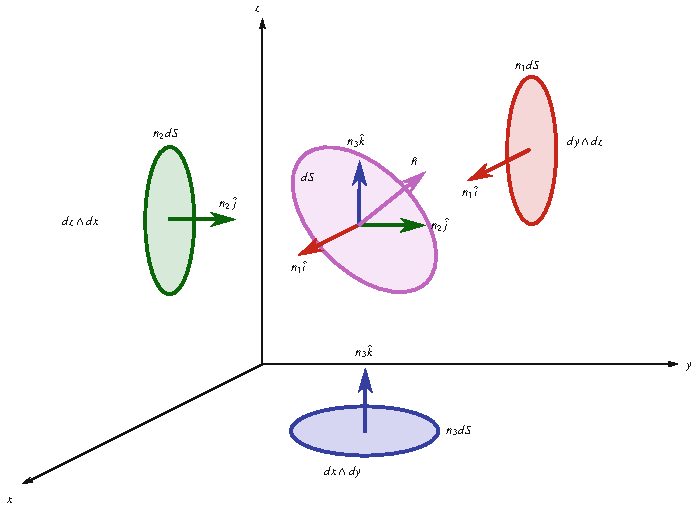
\includegraphics[width=0.960\linewidth]{images/vector/fig-9-18.pdf}
  \caption{带单位法向量 $\hat{n}=n_1\hat{\imath}+n_2\hat{\jmath}+n_3\hat{k}$ 的无穷小面积 $dS$ 被分解为 $n_1dS$、$n_2dS$ 和 $n_3dS$，其单位法向量分别为 $n_1\hat{\imath}$、$n_2\hat{\jmath}$ 和 $n_3\hat{k}$}
  \label{fig:9-18}
\end{figure}

因此我们可以把 $F\cdot\hat{n}\,dS$ 写成 $F\cdot dS$，于是有
\[
\begin{aligned}
\iint_S F\cdot dS&=\iint_S\bigl(P\hat{\imath}+Q\hat{\jmath}+R\hat{k}\bigr)\cdot\bigl(n_1\hat{\imath}+n_2\hat{\jmath}+n_3\hat{k}\bigr)\,dS\\
&=\iint_S(Pn_1+Qn_2+Rn_3)\,dS\\
&=\iint_S\bigl(P\,n_1dS+Q\,n_2dS+R\,n_3dS\bigr)\\
&=\iint_S\bigl(P\,dy\wedge dz+Q\,dz\wedge dx+R\,dx\wedge dy\bigr)\\
&=\iint_S\ast F^{\flat},
\end{aligned}
\]
这正是我们想要证明的. 当我们把 $F$ 替换为 $\operatorname{curl}F$ 时，我们有
\[
\iint_S\operatorname{curl}F\cdot dS=\iint_S\ast(\operatorname{curl}F)^{\flat}=\iint_S d(F^{\flat}).
\]
这样我们就重写了 Stokes 定理的左边. 把右边和左边的部分放在一起，我们可以把向量微积分版本的 Stokes 定理重写为
\[
\iint_S d(F^{\flat})=\oint_{\partial S}F^{\flat}.
\]
显然，$F^{\flat}$ 是一个 1-形式 $\alpha$，而 $S$ 是一个二维流形 $M$，这意味着我们已经把 Stokes 定理写成
\[
\int_M d\alpha=\int_{\partial M}\alpha.
\]

\subsection{散度定理}

最后，我们来看向量微积分中的散度定理，
\[
\iiint_V\operatorname{div}F\,dV=\oint_{\partial V}F\cdot dS.
\]
我们注意到左边的被积函数不是别的，正是 $\ast(\operatorname{div}F)$，它可以重写为 $d\bigl((\ast\circ\flat)F\bigr)$. 我们还看到右边 $\oint_{\partial V}F\cdot dS$ 可以写成 $\oint_{\partial V}\ast(F^{\flat})$. 这使得我们可以把散度定理写成
\[
\iiint_V d\bigl((\ast\circ\flat)F\bigr)=\oint_{\partial V}\ast(F^{\flat}).
\]
把三维流形 $V$ 写成 $M$，把三维 2-形式 $(\ast\circ\flat)F$ 写成 $\alpha$，散度定理就是
\[
\int_M d\alpha=\int_{\partial M}\alpha.
\]
这样我们就用微分形式记号把我们的三个向量微积分定理写成了相同的形式. 这个恒等式
\[
\int_M d\alpha=\int_{\partial M}\alpha
\]
正是我们将在几章之后证明的广义 Stokes 定理.

\section{小结、参考文献与问题}

\subsection{小结}

从几何上讲，散度度量向量场在点 $(x_0,y_0,z_0)$ 处``发散''或``散开''的程度. 给定围绕点 $(x_0,y_0,z_0)$ 的、带边界 $\partial V$ 和体积 $\Delta V$ 的小三维区域 $V$，$F$ 在 $(x_0,y_0,z_0)$ 处的散度定义为
\[
\operatorname{div}F=\lim_{\Delta V\to0}\frac{1}{\Delta V}\oint_{\partial V}F\cdot\hat{n}\,dS.
\]

本质上，旋度度量向量场 $F$ 绕某点无穷小路径的每单位面积的``环流''. 假设 $S$ 是以闭曲线 $C=\partial S$ 为边界的曲面，$\Delta S$ 是该曲面的面积，$\hat{n}$ 是该曲面的单位法向量，$ds$ 中的 $s$ 是无穷小弧长元素，曲面面积 $\Delta S$ 围绕点 $(x_0,y_0,z_0)$ 收缩到零. 那么 $F$ 在点 $(x_0,y_0,z_0)$ 处的旋度定义为
\[
\hat{n}\cdot\operatorname{curl}F=\lim_{|\Delta S|\to0}\frac{1}{\Delta S}\oint_C F\cdot\hat{t}\,ds.
\]

我们基本上是反过来定义函数 $f$ 的梯度：把它定义为与单位长度向量 $u$ 点积后给出 $f$ 沿方向 $u$ 的方向导数的那个向量场，
\[
\operatorname{grad}f\cdot u=u[f].
\]

利用散度、旋度和梯度的这些几何定义，有可能得到向量微积分中的标准公式定义. 令 $F=P\hat{\imath}+Q\hat{\jmath}+R\hat{k}$，我们有
\begin{align*}
\operatorname{div}F=\frac{\partial P}{\partial x}+\frac{\partial Q}{\partial y}+\frac{\partial R}{\partial z}, \\
\operatorname{curl}F=\Bigl(\frac{\partial R}{\partial y}-\frac{\partial Q}{\partial z}\Bigr)\hat{\imath}+\Bigl(\frac{\partial P}{\partial z}-\frac{\partial R}{\partial x}\Bigr)\hat{\jmath}+\Bigl(\frac{\partial Q}{\partial x}-\frac{\partial P}{\partial y}\Bigr)\hat{k}, \\
\operatorname{grad}f=\frac{\partial f}{\partial x}\hat{\imath}+\frac{\partial f}{\partial y}\hat{\jmath}+\frac{\partial f}{\partial z}\hat{k}.
\end{align*}

为了与 Einstein 求和记号保持一致，向量基元素用下指标书写，向量分量用上指标书写. 余向量（微分形式）基元素用上指标书写，余向量（微分形式）分量用下指标书写. 这使我们能够用笛卡尔坐标给出音乐同构. $\flat$ 同构由
\[
\flat:T_pM\longrightarrow T_p^*M,\qquad v^i\frac{\partial}{\partial x^i}\longmapsto v_idx^i,\quad\text{其中 }v_i=v^i
\]
给出，而 $\sharp$ 同构由
\[
\sharp:T_p^*M\longrightarrow T_pM,\qquad \alpha_idx^i\longmapsto\alpha^i\frac{\partial}{\partial x^i},\quad\text{其中 }\alpha^i=\alpha_i
\]
给出. 记住，这些实际上不是音乐同构的数学定义，而只是它们在笛卡尔坐标下的公式. 但连同 Hodge 星算子，这些同构提供了向量微积分与微分形式之间的联系. 下面的图表交换.
\[
\begin{array}{ccccccccc}
C(\mathbb{R}^3)&\xrightarrow{\ \operatorname{grad}\ }&T\mathbb{R}^3&\xrightarrow{\ \operatorname{curl}\ }&T\mathbb{R}^3&\xrightarrow{\ \operatorname{div}\ }&C(\mathbb{R}^3)\\[2pt]
\Big\downarrow \mathrm{id}&&\Big\downarrow \flat&&\Big\downarrow {\ast\circ\flat}&&\Big\downarrow \ast\\[2pt]
\Lambda^0(\mathbb{R}^3)&\xrightarrow{\ \ d\ \ }&\Lambda^1(\mathbb{R}^3)&\xrightarrow{\ \ d\ \ }&\Lambda^2(\mathbb{R}^3)&\xrightarrow{\ \ d\ \ }&\Lambda^3(\mathbb{R}^3)
\end{array}
\]
这使得向量微积分中的下列恒等式可以用外微分写出：
\[
\nabla\times(\nabla f)=0\quad\longleftrightarrow\quad d(df)=0,\qquad
\nabla\cdot(\nabla\times F)=0\quad\longleftrightarrow\quad d(d\alpha)=0.
\]
注意 $d(df)=0$ 和 $d(d\alpha)=0$ 当然只是 Poincaré 引理的推论. 它也使向量微积分中的三个主要定理可以用微分形式写出. 事实上，这三个定理都是微分形式版本 Stokes 定理的特殊情形：
\begin{align*}
f\bigl(c(b)\bigr)-f\bigl(c(a)\bigr)=\int_C\nabla f\cdot ds \\
\Downarrow \\
\int_{\partial C}\alpha=\int_C d\alpha, \\
\oint_{\partial S}F\cdot ds=\iint_S(\nabla\times F)\cdot dS \\
\Downarrow \\
\int_{\partial S}\alpha=\int_S d\alpha, \\
\oint_{\partial V}F\cdot dS=\iiint_V\nabla\cdot F\,dV \\
\Downarrow \\
\int_{\partial V}\alpha=\int_V d\alpha.
\end{align*}

\subsection{参考文献与进一步阅读}

本章前半部分给出的散度、旋度和梯度的几何处理方法，很大程度上受到 Schey~\cite{ref38} 的启发并追随其思路，\cite{ref38} 可能给出了这些向量微积分算子在现有文献中最好、最直观的几何导引. 特别是，关于散度、旋度、梯度和拉普拉斯算子在柱坐标和球坐标下的更详细推导，参见这本书. 散度、旋度和梯度算子与外微分之间的关系几乎在任何地方都有介绍，但特别参见 Abraham、Marsden 和 Ratiu~\cite{ref01}、Hubbard 和 Hubbard~\cite{ref27} 或 Edwards~\cite{ref18}. 音乐同构（升号和降号）例如在 Abraham、Marsden 和 Ratiu~\cite{ref01} 以及 Marsden 和 Ratiu~\cite{ref32} 中引入，另外在 Burke~\cite{ref08} 和 Darling~\cite{ref12} 中也有非常简短的介绍.

\subsection{问题}

\begin{center}
\small
\begin{tabular}{ccc}
$f_1(x,y,z)=5xy^2-4x^3y$ & $f_5(x,y,z)=x^2y^3z^4$ & $f_9(x,y,z)=x^2y^3z-3xyz^2$\\[3pt]
$f_2(x,y,z)=y\ln(z)$ & $f_6(x,y,z)=\sqrt{x+yz}$ & $f_{10}(x,y,z)=x^2+y^2-5z^2$\\[3pt]
$f_3(x,y,z)=\sqrt{1+2xy}$ & $f_7(x,y,z)=xe^y+ye^z+ze^x$ & $f_{11}(x,y,z)=-x^2y-y^3z^2+z^4x^5$\\[3pt]
$f_4(x,y,z)=x^4-x^2y^3$ & $f_8(x,y,z)=xe^{yz}$ & $f_{12}(x,y,z)=3x-4y+5z$
\end{tabular}
\end{center}

\begin{question}\label{q:9-12}
对上面列出的函数求 $\operatorname{grad}f_i$. 再求 $(\operatorname{grad}f_i)^{\flat}$.
\end{question}

\begin{question}\label{q:9-13}
对上面列出的函数求 $df_i$. 并与问题~\ref{q:9-12} 中的 $(\operatorname{grad}f_i)^{\flat}$ 比较.
\end{question}

\begin{question}\label{q:9-14}
对上面列出的函数求 $\operatorname{curl}(\operatorname{grad}f_i)$. 再求 $d(df)$. 比较.
\end{question}

\begin{center}
{\setlength{\tabcolsep}{4pt}\small\begin{tabular}{ccc}
$F_1=2x^2\hat{\imath}+(x+y)\hat{\jmath}$ & $F_5=x^2\hat{\imath}+xy\hat{\jmath}-(x^2+y^2+z^2)\hat{k}$ & $F_9=e^{xy}\hat{\imath}-e^{yz}\hat{\jmath}+e^{xz}\hat{k}$\\[3pt]
$F_2=-x\hat{\imath}+(x-2y)\hat{\jmath}$ & $F_6=yz^2\hat{\imath}+yz\hat{\jmath}+(2x-2y)\hat{k}$ & $F_{10}=\sqrt{xyz}\,\hat{\imath}+\sqrt{xy}\,\hat{\jmath}+\sqrt{x}\,\hat{k}$\\[3pt]
$F_3=2x^2\hat{\imath}-3y^3\hat{\jmath}$ & $F_7=y\hat{\imath}+z\hat{\jmath}+x\hat{k}$ & $F_{11}=xy^2z\hat{\imath}-2x^2y^3z\hat{\jmath}+3xy^3z^2\hat{k}$\\[3pt]
$F_4=3\hat{\jmath}+4\hat{k}$ & $F_8=-x^2\hat{\imath}+y^3\hat{\jmath}-z^4\hat{k}$ & $F_{12}=y^2\hat{\imath}+(e^x+e^y)\hat{\jmath}-(x^3-2y)\hat{k}$
\end{tabular}}
\end{center}

\begin{question}\label{q:9-15}
对上面列出的向量求 $\operatorname{curl}F_i$. 再求 $(\ast\circ\flat)(\operatorname{curl}F_i)$.
\end{question}

\begin{question}\label{q:9-16}
对上面列出的向量求 $F_i^{\flat}$. 再求 $d(F_i^{\flat})$. 并与问题~\ref{q:9-15} 中的 $(\ast\circ\flat)(\operatorname{curl}F_i)$ 比较.
\end{question}

\begin{question}\label{q:9-17}
对上面列出的向量求 $\operatorname{div}(\operatorname{curl}F_i)$. 再求 $d\bigl(dF_i^{\flat}\bigr)$. 比较.
\end{question}

\begin{center}
{\setlength{\tabcolsep}{3pt}\footnotesize\begin{tabular}{ccc}
$G_1=-x^2y\hat{\imath}-xy^2\hat{\jmath}$ & $G_5=\sqrt{xy}\,\hat{\imath}+xy\hat{\jmath}+(3x+2y+z)\hat{k}$ & $G_9=e^{xy}\hat{\imath}-e^{yz}\hat{\jmath}+e^{xz}\hat{k}$\\[3pt]
$G_2=(x+2y)\hat{\imath}+2xy\hat{\jmath}$ & $G_6=yz^2\hat{\imath}+yz\hat{\jmath}-(x^2+y^2+z^2)\hat{k}$ & $G_{10}=x^3yz\hat{\imath}+x^2y\hat{\jmath}+\sqrt{x}\,\hat{k}$\\[3pt]
$G_3=x^2y^2\hat{\imath}-3x^2y^2\hat{\jmath}$ & $G_7=\sqrt{yz}\,\hat{\imath}+\sqrt{xz}\,\hat{\jmath}+\sqrt{xy}\,\hat{k}$ & $G_{11}=3xyz\hat{\imath}+\sqrt{xyz}\,\hat{\jmath}+(4y-z)\hat{k}$\\[3pt]
$G_4=3x\hat{\jmath}+4y\hat{k}$ & $G_8=e^x\hat{\imath}+e^y\hat{\jmath}-e^z\hat{k}$ & $G_{12}=(x^2+y^2+z^2)\hat{\imath}+3x\hat{\jmath}-e^{xyz}\hat{k}$
\end{tabular}}
\end{center}

\begin{question}\label{q:9-18}
对上面列出的向量求 $\operatorname{div}(G_i)$. 再求 $\ast(\operatorname{div}G_i)$.
\end{question}

\begin{question}\label{q:9-19}
对上面列出的向量求 $(\ast\circ\flat)G_i$. 再求 $d\bigl((\ast\circ\flat)G_i\bigr)$. 并与问题~\ref{q:9-18} 中的 $\ast(\operatorname{div}G_i)$ 比较.
\end{question}

\begin{question}\label{q:9-20}
求一个函数 $f$，使得 $\nabla f=xy^2\hat{\imath}+x^2y\hat{\jmath}$，然后用这个函数和线积分基本定理计算 $\int_C\nabla f\cdot ds$，其中曲线 $C$ 由 $\gamma(t)=\bigl(t+\sin\frac{\pi t}{2},\,t+\cos\frac{\pi t}{2}\bigr)$、$0\leq t\leq1$ 给出. 用微分形式写出这个积分.
\end{question}

\begin{question}\label{q:9-21}
求一个函数 $f$，使得 $\nabla f=yz\hat{\imath}+xz\hat{\jmath}+(xy+2z)\hat{k}$，然后用这个函数和线积分基本定理计算 $\int_C\nabla f\cdot ds$，其中积分沿从 $(1,0,-2)$ 到 $(4,6,3)$ 的线段.
\end{question}

\begin{question}\label{q:9-22}
求一个函数 $f$，使得 $\nabla f=(2xz+y^2)\hat{\imath}+2xy\hat{\jmath}+(x^2+3z^2)\hat{k}$，然后用这个函数和线积分基本定理计算 $\int_C\nabla f\cdot ds$，其中曲线 $C$ 由 $\gamma(t)=(t^2,t+1,2t-1)$、$0\leq t\leq1$ 给出. 用微分形式写出这个积分.
\end{question}

\begin{question}\label{q:9-23}
求一个函数 $f$，使得 $\nabla f=y^2\cos(z)\hat{\imath}+2xy\cos(z)\hat{\jmath}-xy^2\sin(z)\hat{k}$，然后用这个函数和线积分基本定理计算 $\int_C\nabla f\cdot ds$，其中曲线 $C$ 由 $\gamma(t)=(t^2,\sin t,t)$、$0\leq t\leq\pi$ 给出. 用微分形式写出这个积分.
\end{question}

\begin{question}\label{q:9-24}
用 Stokes 定理计算 $\iint_S(\nabla\times F)\cdot dS$，其中 $F=2y\cos(z)\hat{\imath}+e^x\sin(z)\hat{\jmath}+xe^y\hat{k}$，$S$ 是球面 $x^2+y^2+z^2=16$、$z\geq0$ 朝上定向的部分. 然后用微分形式写出这个积分.
\end{question}

\begin{question}\label{q:9-25}
用 Stokes 定理计算 $\iint_S(\nabla\times F)\cdot dS$，其中 $F=e^{xy}\cos(z)\hat{\imath}+x^2z\hat{\jmath}+xy\hat{k}$，$S$ 是半球面 $x=\sqrt{1-y^2-z^2}$，按正 $x$ 轴方向定向. 然后用微分形式写出这个积分.
\end{question}

\begin{question}\label{q:9-26}
用 Stokes 定理计算 $\oint_C F\cdot ds$，其中 $F=yz\hat{\imath}+2xz\hat{\jmath}+e^{xy}\hat{k}$，$C$ 是平面 $z=4$ 中的圆 $x^2+y^2=9$. $C$ 从上方看时按逆时针定向. 然后用微分形式写出这个积分.
\end{question}

\begin{question}\label{q:9-27}
用散度定理计算曲面积分 $\iint_S F\cdot dS$，其中 $F=x^2z^3\hat{\imath}+2xyz^3\hat{\jmath}+xz^4\hat{k}$，$S$ 是顶点为 $(\pm3,\pm2,\pm2)$ 的盒子的表面. 然后用微分形式写出这个积分.
\end{question}

\begin{question}\label{q:9-28}
用散度定理计算曲面积分 $\iint_S F\cdot dS$，其中 $F=e^x\sin(y)\hat{\imath}+e^x\cos(y)\hat{\jmath}+yz^2\hat{k}$，$S$ 是由平面 $x=0$、$x=1$、$y=0$、$y=1$、$z=0$、$z=1$ 围成的盒子的表面. 然后用微分形式写出这个积分.
\end{question}

\begin{question}\label{q:9-29}
用散度定理计算曲面积分 $\iint_S F\cdot dS$，其中 $F=3xy^2\hat{\imath}+xe^z\hat{\jmath}+z^3\hat{k}$，$S$ 是由平面 $x=-1$、$x=1$ 和柱面 $y^2+z^2=4$ 围成的立体的表面. 然后用微分形式写出这个积分.
\end{question}
